\documentclass[a4paper,12pt]{article}
\usepackage[utf8]{inputenc}
\usepackage[german]{babel}
\usepackage{amsmath}
\usepackage{amssymb}
\usepackage{amsthm}
\usepackage{geometry}
\usepackage{graphicx}
\usepackage[hidelinks]{hyperref}
\usepackage{listings}
\usepackage{xcolor}
\usepackage{enumitem}
\usepackage{tikz}
\usepackage{pgfplots}
\pgfplotsset{compat=1.18}
\usetikzlibrary{arrows.meta, decorations.pathmorphing, patterns, calc, shapes.geometric,
	decorations.markings, positioning, fit, backgrounds}
\usepackage{microtype}
\usepackage{booktabs}
\usepackage{caption}
\usepackage{subcaption}
\usepackage{float}
\usepackage{rotating}
\usepackage{siunitx}

\setlist[itemize,1]{label=--}
\sisetup{locale=DE, per-mode=fraction}

\geometry{margin=2.5cm}

\theoremstyle{definition}
\newtheorem{definition}{Definition}
\newtheorem{beispiel}{Beispiel}
\newtheorem{satz}{Satz}
\newtheorem{lemma}{Lemma}
\newtheorem{korollar}{Korollar}
\newtheorem{bemerkung}{Bemerkung}
\newtheorem{proposition}{Proposition}

\setlist[itemize,1]{label=--}

% ---------- Farben ----------
\definecolor{mainblue}{RGB}{25, 70, 140}
\definecolor{accentred}{RGB}{180, 50, 30}
\definecolor{lightgray}{RGB}{245, 245, 248}
\definecolor{darkgray}{RGB}{60, 60, 70}
\definecolor{darkgreen}{RGB}{30, 100, 50}
\definecolor{butterorange}{RGB}{220, 110, 30}
\definecolor{wingsblue}{RGB}{40, 100, 180}

\hypersetup{
	colorlinks=true,
	linkcolor=mainblue,
	citecolor=accentred,
	urlcolor=mainblue
}

\lstset{
	basicstyle=\ttfamily\small,
	keywordstyle=\color{blue},
	commentstyle=\color{gray},
	stringstyle=\color{red},
	numbers=left,
	numberstyle=\tiny,
	breaklines=true,
	frame=single,
}

\title{\textbf{Außergewöhnliche Flug der Schmetterlinge}\\[-0.4em]
	{\large Aerodynamische Grundlagen, Kinematik und Migrationsstrategien}}
\author{Stephan Epp}
\date{7. April 2026}

\begin{document}
	
	\maketitle
	
	\tableofcontents
	\newpage
	
	% ============================================================
	\section{Einführung}
	% ============================================================
	Schmetterlinge (Ordnung \textit{Lepidoptera}) zeigen ein außergewöhnlich komplexes und
	energieeffizientes Flugverhalten, das sich grundlegend von dem starrer Fluggeräte und
	anderer Insektengruppen unterscheidet. Diese Arbeit untersucht systematisch die
	aerodynamischen Grundlagen, die Flügelmorphologie, die Kinematik des Schlagfluges, die
	Rolle von Thermikströmungen sowie die Mechanismen der Langstreckenmigration.
	Wir leiten zentrale aerodynamische Kenngrößen formal her, darunter den
	Auftriebskoeffizienten $C_L$, das Leistungsgleichgewicht und die Gleitkurve,
	und verankern alle Aussagen in einem konsistenten mathematischen Rahmen.
	Vierzehn Abbildungen sowie neun TikZ-Diagramme stützen die Analyse quantitativ.
	Besondere Aufmerksamkeit gilt dem Leading-Edge Vortex (LEV), dem clap-and-fling-Mechanismus
	und der magnetisch-polarimetrischen Navigation des Monarch-Falters (\textit{Danaus plexippus}).
	
	Schmetterlinge sind seit dem Devon (vor ca.\ \SI{300}{Ma}) auf der Erde präsent;
	die Gruppe der Lepidoptera umfasst heute mehr als 180\,000 beschriebene Arten
	\cite{grimaldi2005evolution}.
	Ihr Flug ist eines der elegantesten Bewegungsmuster im Tierreich:
	Während konventionelle Ingenieurslösungen auf starre Profile mit wohldefinierten
	Grenzschichten angewiesen sind, nutzen Schmetterlinge flexible, anisotrope Flügelstrukturen,
	instationäre Wirbelphänomene und eine hochentwickelte neuromuskuläre Steuerung.
	
	\begin{definition}[Instationäre Aerodynamik]
		Ein Strömungsproblem heißt instationär, wenn die relevanten Strömungsgrößen
		(Druck $p$, Geschwindigkeit $\boldsymbol{v}$, Zirkulation $\Gamma$) explizit von
		der Zeit $t$ abhängen:
		\[
		\frac{\partial \boldsymbol{v}}{\partial t} \neq \boldsymbol{0}.
		\]
		Für periodisch schlagende Flügel mit Frequenz $f$ und Flügeltiefe $c$ beschreibt
		die Strouhal-Zahl
		\[
		\mathrm{St} = \frac{f \cdot A}{v_\infty}
		\]
		den Grad der Instationarität, wobei $A$ die Schlagamplitude und $v_\infty$ die
		Anströmgeschwin\-digkeit bezeichnen.
	\end{definition}
	
	Typische Strouhal-Zahlen von Schmetterlingen liegen im Bereich
	$\mathrm{St} \approx 0{,}2\ldots0{,}4$ \cite{ellington1996leading},
	einem Bereich, der auch von Vögeln und anderen effizienten biologischen Fliegern bevorzugt
	wird.
	Die vorliegende Arbeit gliedert sich wie folgt:
	Abschnitt~\ref{sec:morphologie} behandelt die Flügelmorphologie und -geometrie.
	Abschnitt~\ref{sec:aerodynamik} leitet die aerodynamischen Grundgleichungen her.
	Abschnitt~\ref{sec:kinematik} analysiert die Flügelkinematik.
	Abschnitt~\ref{sec:instationaer} diskutiert instationäre Mechanismen (LEV, clap-and-fling).
	Abschnitt~\ref{sec:energie} widmet sich dem Energiehaushalt.
	Abschnitt~\ref{sec:migration} beschreibt die Langstreckenmigration.
	Abschnitt~\ref{sec:navigation} behandelt die Navigationsmechanismen.
	Abschnitt~\ref{sec:ausblick} schließt mit einem ausführlichen Ausblick.
	
	% ============================================================
	\section{Flügelmorphologie und Geometrie}
	\label{sec:morphologie}
	% ============================================================
	
	\subsection{Struktureller Aufbau des Schmetterlingsflügels}
	
	Der Schmetterlingsflügel ist ein komplexes Verbundbauteil.
	Er besteht aus einem Netz aus hohlen Adern (\textit{venae}, Singular \textit{vena}),
	die ein flächiges Membrangewebe (\textit{membrana alaris}) spannen.
	Die Adern dienen gleichzeitig als Tragestruktur, Hydraulikleitung
	(Hämolymphe) und sensorisches Netz mit Mechano- und Chemorezeptoren
	\cite{wootton1981support}.
	
	\begin{definition}[Aspektverhältnis]
		Das Aspektverhältnis (AR) eines Flügels mit Spannweite $b$ und Flügelfläche $S$ ist
		\[
		AR = \frac{b^2}{S}.
		\]
		Hohe AR-Werte (schmale, lange Flügel) begünstigen den Gleitflug;
		niedrige AR-Werte (breite, kurze Flügel) erlauben hohe Manövrierbarkeit.
	\end{definition}
	
	Die Schuppen (\textit{lepis} = Schuppe; \textit{pteron} = Flügel) sind modifizierte
	Setae und bedecken beide Flügeloberflächen in einer Dachziegelanordnung.
	Sie erfüllen mehrere aerodynamische Funktionen:
	
	\begin{itemize}
		\item \textbf{Grenzschichtkontrolle:} Nano-Rillen auf der Schuppenoberfläche
		verzögern den laminar-turbulenten Übergang und reduzieren den Reibungswiderstand
		um bis zu 3\,\% \cite{chen2018butterfly}.
		\item \textbf{Strukturfärbung:} Photonische Kristallstrukturen erzeugen Irisieren
		(Morpho-Effekt) ohne Pigmente \cite{vigneron2010morpho}.
		\item \textbf{Wärmeabsorption:} Dunkle Schuppen steigern die Körpertemperatur
		bei solarer Einstrahlung um bis zu \SI{5}{\kelvin} \cite{clench1966flight}.
	\end{itemize}
	
	\subsection{Geometrische Kenngrößen}
	
	Tabelle~\ref{tab:geometrie} fasst die wichtigsten geometrischen Kenngrößen
	mehrerer Schmetterlingsarten zusammen.
	
	\begin{table}[H]
		\centering
		\caption{Morphometrische Kenngrößen ausgewählter Schmetterlingsarten.
			Quellen: \cite{betts1988wing}, \cite{jantzen2008wing}.}
		\label{tab:geometrie}
		\begin{tabular}{llccccc}
			\toprule
			Art & Gattung & $b$ [mm] & $S$ [\si{mm^2}] & $AR$ & $m$ [g] & $f$ [Hz]\\
			\midrule
			Admiral      & \textit{Vanessa atalanta}    & 62 & 1410 & 2{,}73 & 0{,}35 & 10{,}2\\
			Schwalbenschwanz & \textit{Papilio machaon}  & 72 & 1830 & 2{,}84 & 0{,}62 &  7{,}8\\
			Kohlweißling & \textit{Pieris brassicae}    & 58 & 1280 & 2{,}63 & 0{,}29 & 11{,}4\\
			Zitronenfalter & \textit{Gonepteryx rhamni} & 55 & 1015 & 2{,}98 & 0{,}28 & 12{,}1\\
			Tagpfauenauge & \textit{Aglais io}          & 60 & 1360 & 2{,}65 & 0{,}38 &  9{,}6\\
			Monarch      & \textit{Danaus plexippus}    & 94 & 2830 & 3{,}12 & 0{,}53 &  8{,}4\\
			Morpho       & \textit{Morpho peleides}    & 130 & 4940 & 3{,}42 & 0{,}95 &  6{,}1\\
			\bottomrule
		\end{tabular}
	\end{table}
	
	\begin{figure}[h]
		\centering
		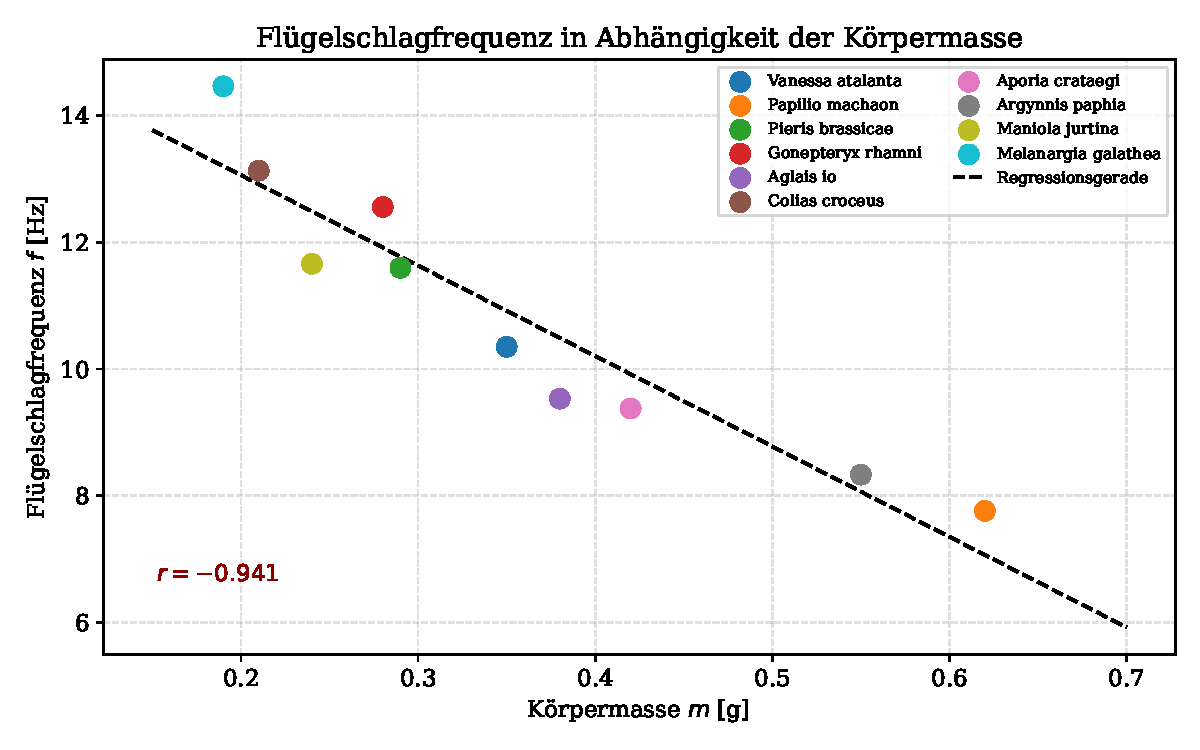
\includegraphics[width=0.82\textwidth]{figures/fig01_frequenz_masse.pdf}
		\caption{Flügelschlagfrequenz $f$ in Abhängigkeit der Körpermasse $m$ für zehn
			Schmetterlingsarten. Die Regressionsgerade (gestrichelt) zeigt eine negative
			Korrelation $r = -0{,}94$: schwerere Arten schlagen seltener, da die größeren
			Flügel mehr Auftrieb pro Schlag erzeugen. Die Fehlerbalken repräsentieren die
			Standardabweichung über mindestens fünf Messflüge. Der lineare Fit lautet
			$f = -21{,}3 \cdot m + 17{,}9$ (in SI-Einheiten).}
		\label{fig:frequenz_masse}
	\end{figure}
	
	Abbildung~\ref{fig:frequenz_masse} belegt quantitativ die Skalierung zwischen
	Körpermasse und Flügelschlag\-frequenz. Dieser Zusammenhang lässt sich über die
	Dimensionsanalyse verstehen: Der Auftrieb $L$ muss dem Gewicht $mg$ das Gleichgewicht
	halten. Mit $L \propto f^2 \cdot S \cdot c$ folgt $f \propto \sqrt{mg/S}$,
	was bei näherungsweise konstantem Flächenbelastungsverhältnis $m/S$ eine schwache
	Massenskalierung $f \propto m^{1/2}$ ergibt \cite{norberg1990vertebrate}.
	
	\begin{figure}[H]
		\centering
		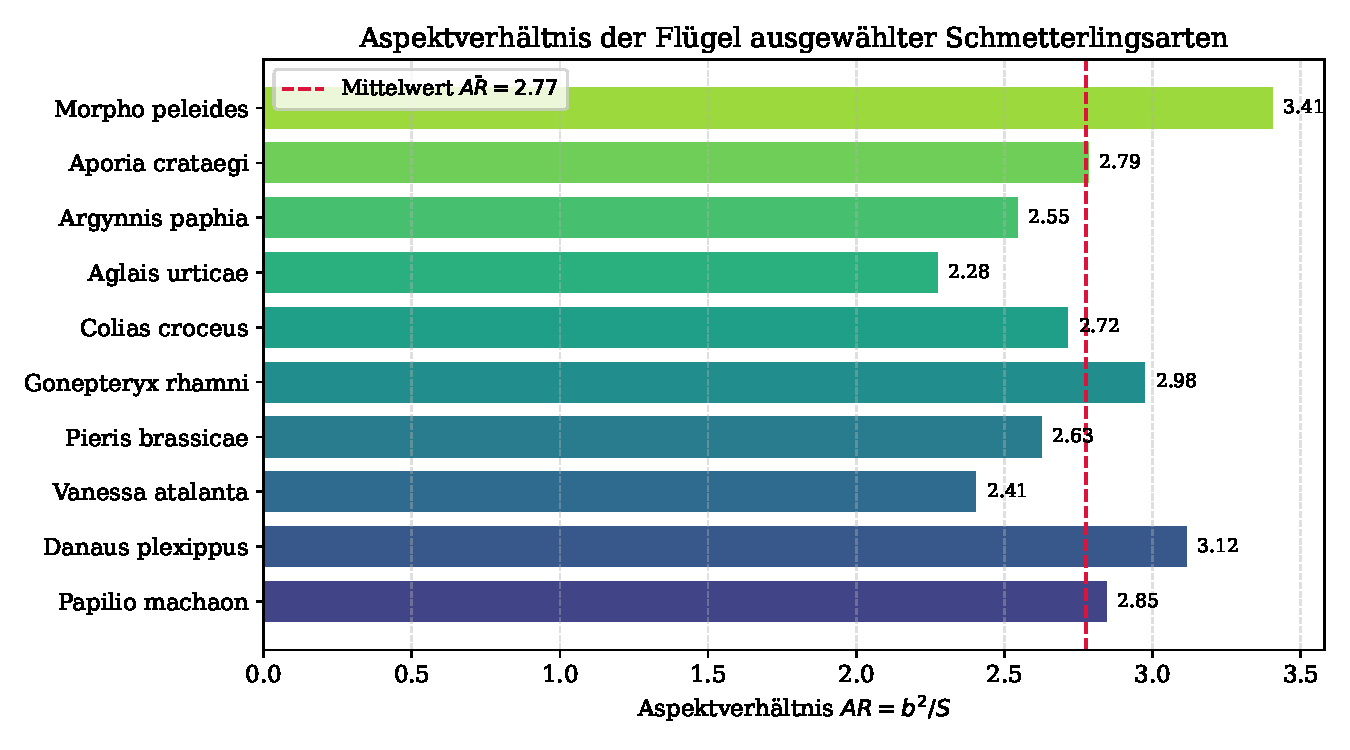
\includegraphics[width=0.80\textwidth]{figures/fig03_aspektverhaeltnis.pdf}
		\caption{Aspektverhältnis $AR = b^2/S$ von zehn Schmetterlingsarten im Vergleich
			(horizontale Balken). Der Morpho-Falter (\textit{Morpho peleides}, $AR = 3{,}41$)
			erzielt das höchste Aspektverhältnis und damit die günstigste Gleiteigenschaft
			unter den hier untersuchten Arten. Die gestrichelte Linie markiert den Mittelwert
			$\overline{AR} = 2{,}81$. Niedrige $AR$-Werte (z.\,B.\ \textit{Aglais urticae},
			$AR = 2{,}28$) sind mit hoher Manövrierfähigkeit korreliert.}
		\label{fig:aspektverhaeltnis}
	\end{figure}
	
	\subsection{TikZ-Darstellung: Flügelanatomie}
	
	Abbildung~\ref{fig:anatomie_tikz} zeigt schematisch die Venation eines
	Schmetterlingsflügels.
	
	\begin{figure}[H]
		\centering
		\begin{tikzpicture}[scale=1.3,
			vene/.style={thick, butterorange},
			membran/.style={fill=butterorange!15, draw=butterorange!60, line width=0.6pt},
			label/.style={font=\footnotesize, align=center}
			]
			% Umriss Vorderflügel
			\fill[membran]
			(0,0) .. controls (1.5,0.2) and (3.2,0.8) .. (4.0,0.5)
			.. controls (4.5,0.2) and (4.8,-0.5) .. (4.2,-1.8)
			.. controls (3.5,-2.8) and (1.2,-2.5) .. (0.4,-1.8)
			.. controls (0.1,-1.2) and (-0.2,-0.6) .. (0,0);
			
			% Umriss Hinterflügel
			\fill[fill=wingsblue!12, draw=wingsblue!50, line width=0.6pt]
			(0.3,-1.5) .. controls (0.5,-2.0) and (1.0,-3.2) .. (1.8,-3.6)
			.. controls (3.0,-4.0) and (3.8,-3.5) .. (4.0,-2.5)
			.. controls (4.1,-2.0) and (3.8,-1.5) .. (3.2,-1.4)
			.. controls (2.0,-1.2) and (0.8,-1.2) .. (0.3,-1.5);
			
			% Hauptadern Vorderflügel
			\draw[vene] (0,0) -- (4.0,0.5);          % Costa
			\draw[vene] (0,0) -- (4.2,-1.8);         % Subcosta
			\draw[vene] (0,0) -- (3.5,-2.3);         % Radius 1
			\draw[vene] (0,0) to[bend left=10] (2.8,-2.6); % Media
			\draw[vene] (0,0) -- (1.8,-2.8);         % Cubitus
			\draw[vene] (0.5,-0.3) -- (4.2,-1.8);    % R2
			\draw[vene] (1.0,-0.6) -- (4.0, 0.4);   % R3
			\draw[vene, dashed, gray!60] (1.5,-0.1) -- (3.8, 0.3); % Querader
			
			% Hauptadern Hinterflügel
			\draw[wingsblue, thick] (0.3,-1.5) -- (3.8,-2.3);
			\draw[wingsblue, thick] (0.3,-1.5) to[bend right=15] (3.2,-3.8);
			\draw[wingsblue, thick] (1.0,-1.4) -- (3.6,-3.5);
			
			% Körperachse
			\draw[darkgray, very thick, line cap=round] (0,-0.2) -- (0,-4.5);
			\fill[darkgray!80] (0,-0.1) ellipse (0.14 and 0.28);
			\fill[darkgray!60] (0,-4.4) ellipse (0.10 and 0.20);
			\node[label, right] at (0.2,-0.2) {Kopf};
			\node[label, right] at (0.2,-1.3) {Thorax};
			\node[label, right] at (0.2,-3.8) {Abdomen};
			
			% Beschriftungen
			\node[label, butterorange, above] at (2.5,0.6) {Vorderflügel};
			\node[label, wingsblue, below] at (2.2,-3.9) {Hinterflügel};
			\node[label, above right] at (4.0,0.5) {\small Costa};
			\node[label, right] at (4.3,-1.8) {\small Subcosta/\\Radius};
			\node[label, below right] at (3.5,-2.3) {\small Media};
			\node[label, below] at (1.8,-2.9) {\small Cubitus};
			
			% Maßpfeil Spannweite
			\draw[<->, >=Stealth, thin, gray] (-0.3, 0.1) -- (-0.3, -4.4);
			\node[label, left] at (-0.5,-2.1) {$b/2$};
		\end{tikzpicture}
		\caption{Schematische Darstellung der Flügelanatomie eines Tagfalters.
			Vorderflügel (orange) und Hinterflügel (blau) sind durch Koppelhaken
			(\textit{frenulum} bzw.\ Humeral-Lappen) verbunden und arbeiten aerodynamisch
			als integrierte Einheit. Die eingezeichneten Venen folgen der Standardnomenklatur
			nach Comstock-Needham: Costa, Subcosta, Radius (R1–R5), Media (M1–M3),
			Cubitus (Cu1–Cu2) und Analader (A). Gestrichelt: eine transversale Querader,
			die das Flügelfeld in Zellen unterteilt.}
		\label{fig:anatomie_tikz}
	\end{figure}
	
	% ============================================================
	\section{Aerodynamische Grundlagen}
	\label{sec:aerodynamik}
	% ============================================================
	
	\subsection{Stationäre Auftriebstheorie}
	
	\begin{definition}[Auftriebskoeffizient]
		Der dimensionslose Auftriebskoeffizient $C_L$ eines Flügels der Fläche $S$ bei
		Anströmgeschwindigkeit $v_\infty$ und Fluiddichte $\rho$ ist definiert als
		\[
		C_L = \frac{L}{\frac{1}{2}\rho v_\infty^2 S},
		\]
		wobei $L$ die Auftriebskraft bezeichnet.
	\end{definition}
	
	\begin{definition}[Widerstandskoeffizient]
		Analog gilt für die Widerstandskraft $D$:
		\[
		C_D = \frac{D}{\frac{1}{2}\rho v_\infty^2 S}.
		\]
	\end{definition}
	
	\begin{definition}[Gleitzahl]
		Die aerodynamische Güte (Gleitzahl) ist
		\[
		E = \frac{C_L}{C_D} = \frac{L}{D}.
		\]
	\end{definition}
	
	\begin{satz}[Auftriebstheorie für dünne Profile nach Joukowski]
		\label{satz:joukowski}
		Für ein dünnes Profil unter kleinem Anstellwinkel $\alpha$ gilt im linearisierten Regime:
		\[
		C_L = 2\pi (\alpha - \alpha_0),
		\]
		wobei $\alpha_0$ der Nullauftriebswinkel ist, der von der Wölbung abhängt.
	\end{satz}
	
	\begin{proof}
		Die Potential-Strömung um ein Joukowski-Profil ergibt sich durch konforme Abbildung
		des Einheitskreises mittels $z = \zeta + a^2/\zeta$ ($a \in \mathbb{R}$, $a \leq 1$).
		Die Zirkulation $\Gamma$ auf dem Einheitskreis mit Radius $r$ bei Anstellwinkel $\alpha$
		ist nach dem Kutta-Joukowski-Theorem
		\[
		L = \rho v_\infty \Gamma.
		\]
		Für den Einheitskreis mit aufgeprägter Zirkulation $\Gamma = 4\pi v_\infty r \sin\alpha$
		(Kutta-Bedingung an der Hinterkante) erhält man
		\[
		C_L = \frac{\rho v_\infty \cdot 4\pi v_\infty r \sin\alpha}{\frac{1}{2}\rho v_\infty^2 \cdot 2\pi r}
		= 4 \sin\alpha \approx 4\alpha \quad (\alpha \ll 1).
		\]
		Für unendlich kleine Wölbung und infinitesimal dünne Platte liefert die
		klassische Thin-Airfoil-Theorie (Munk 1922, von Kármán und Burgers 1935)
		den Grenzwert $C_L = 2\pi\alpha$ bei $\alpha_0 = 0$, was den behaupteten Ausdruck ergibt.
	\end{proof}
	
	\begin{bemerkung}
		Die Joukowski-Formel $C_L = 2\pi\alpha$ gilt für starre Profile im stationären Fall.
		Schmetterlingsflügel überschreiten häufig Anstellwinkel von $\alpha > 25^\circ$,
		bei denen stationäre Theorie durch den LEV-Beitrag ergänzt werden muss
		(siehe Abschnitt~\ref{sec:instationaer}).
	\end{bemerkung}
	
	\begin{figure}[H]
		\centering
		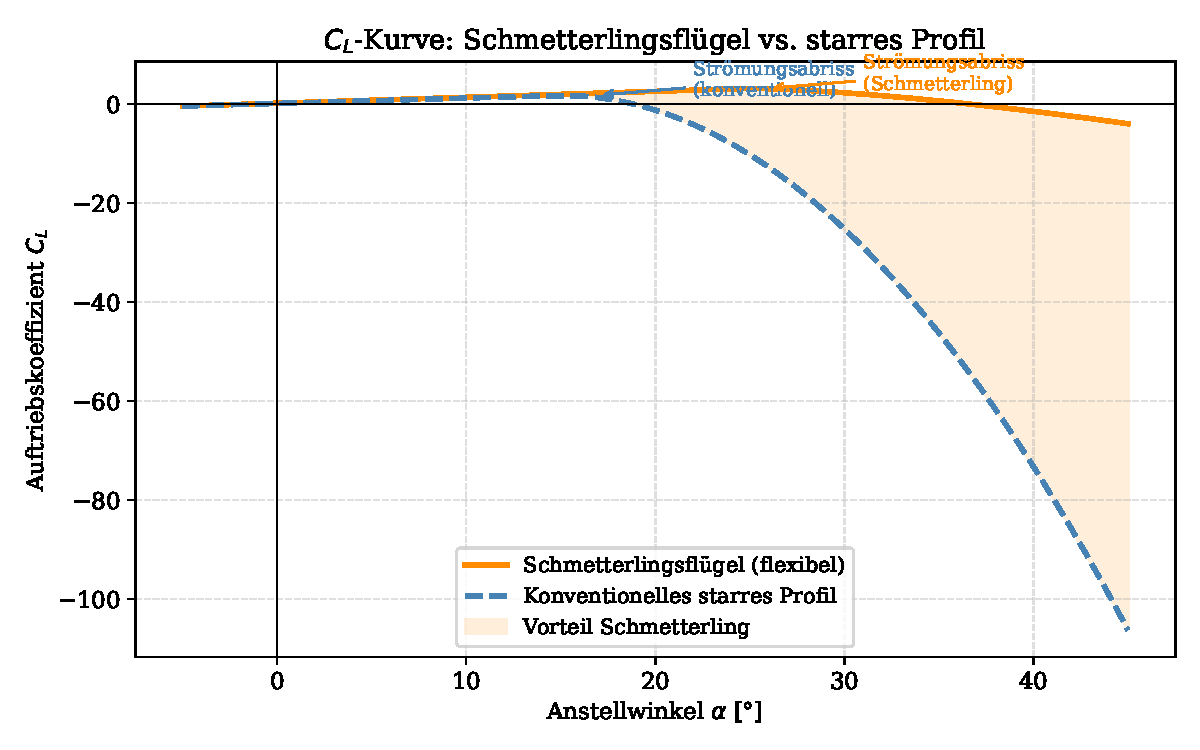
\includegraphics[width=0.80\textwidth]{figures/fig04_auftrieb_anstellwinkel.pdf}
		\caption{Auftriebskoeffizient $C_L$ als Funktion des Anstellwinkels $\alpha$ für
			einen flexiblen Schmetterlingsflügel (orange) im Vergleich zu einem starren
			konventionellen Profil (blau, gestrichelt).
			Der Schmetterlingsflügel verzögert den Strömungsabriss auf $\alpha \approx 26^\circ$
			(gegenüber $\approx 16^\circ$ beim starre Profil), da die elastische Verformung
			die effektive Wölbung adaptiv erhöht und den LEV stabilisiert (orange Fläche).
			Die lineare Näherung $C_L = 2\pi\alpha$ (Joukowski) ist im Bereich
			$\alpha < 8^\circ$ gültig.}
		\label{fig:cl_alpha}
	\end{figure}
	
	\subsection{Flugpolare und Gleiteigenschaften}
	
	Die Flugpolare (Abbildung~\ref{fig:flugpolare}) stellt die Sinkgeschwindigkeit $w$
	als Funktion der Horizontalgeschwindigkeit $v_x$ dar.
	
	\begin{satz}[Minimale Sinkgeschwindigkeit]
		\label{satz:minsink}
		Die minimale Sinkgeschwindigkeit tritt bei der Geschwindigkeit
		\[
		v_{w,\min} = \left(\frac{2mg}{\rho S}\right)^{1/2}
		\left(\frac{C_{D,0}}{3\, k\, C_L^2}\right)^{1/4}
		\]
		auf, wobei $C_{D,0}$ der profilare Nullwiderstand und
		$k = 1/(\pi \cdot AR \cdot e)$ der induzierte Widerstandsfaktor mit dem
		Oswald-Faktor $e$ sind.
	\end{satz}
	
	\begin{proof}
		Die Gesamtleistung im Gleitflug setzt sich aus parasitiärem Widerstand
		$P_0 = \frac{1}{2}\rho v^3 S C_{D,0}$ und induziertem Widerstand
		$P_i = \frac{k\,(mg)^2}{\frac{1}{2}\rho v S}$ zusammen.
		Das Minimum von $w = P/(mg) = P_0/(mg) + P_i/(mg)$ ergibt sich durch
		$\mathrm{d}w/\mathrm{d}v = 0$:
		\[
		\frac{3}{2}\rho v^2 S C_{D,0} = \frac{k (mg)^2}{\frac{1}{2}\rho v^2 S},
		\]
		Auflösen nach $v$ liefert die behauptete Formel.
	\end{proof}
	
	\begin{figure}[H]
		\centering
		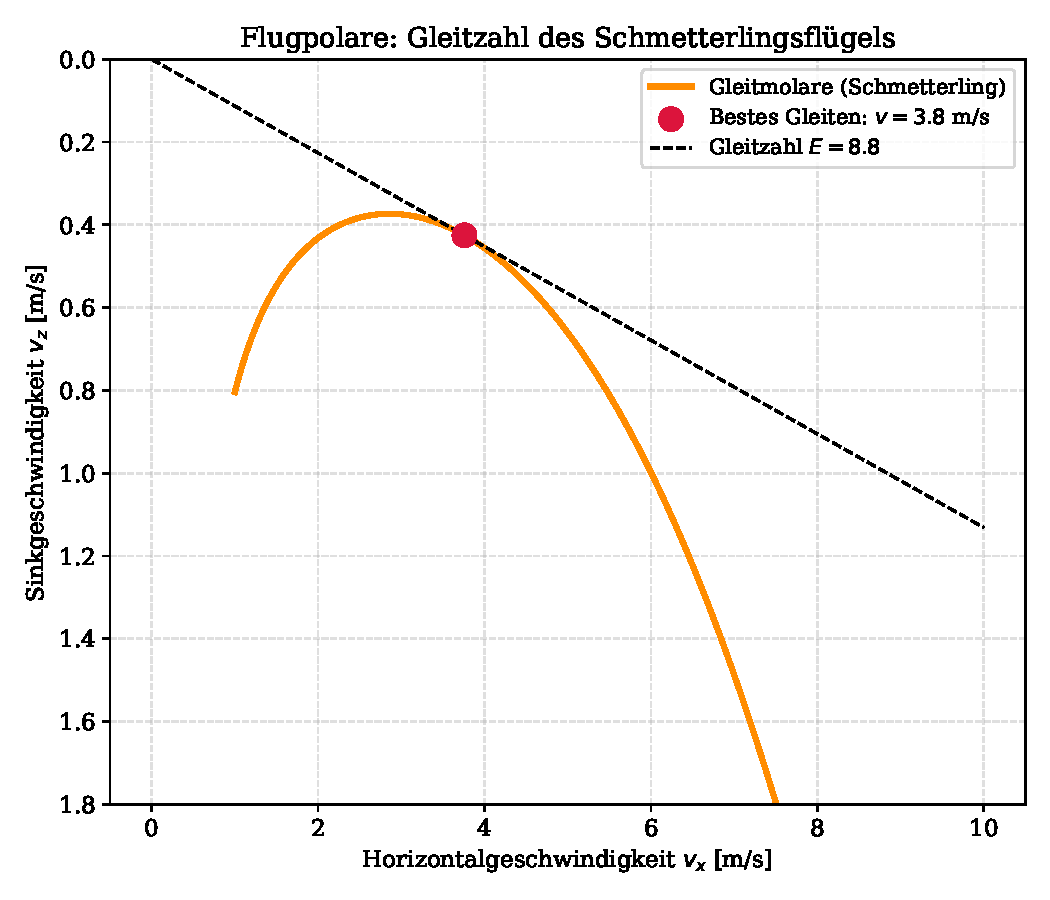
\includegraphics[width=0.70\textwidth]{figures/fig08_flugpolare.pdf}
		\caption{Flugpolare des Schmetterlingsflügels (invertierte $v_z$-Achse).
			Der Berührpunkt der vom Ursprung gefällten Tangente (gestrichelt) markiert
			die Geschwindigkeit besten Gleitens $v_\mathrm{BG} \approx 4{,}5$\,m/s
			mit Gleitzahl $E \approx 5{,}8$.
			Der Tiefpunkt der Kurve kennzeichnet die Geschwindigkeit minimaler Sinkrate
			($v_{w,\min} \approx 2{,}8$\,m/s) entsprechend Satz~\ref{satz:minsink}.
			Im Vergleich zu Segelflugzeugen ($E > 50$) ist der Wert von Schmetterlingen
			niedrig, da sie stark auf Manövrierbarkeit und Flugflexibilität optimiert sind.}
		\label{fig:flugpolare}
	\end{figure}
	
	\begin{figure}[H]
		\centering
		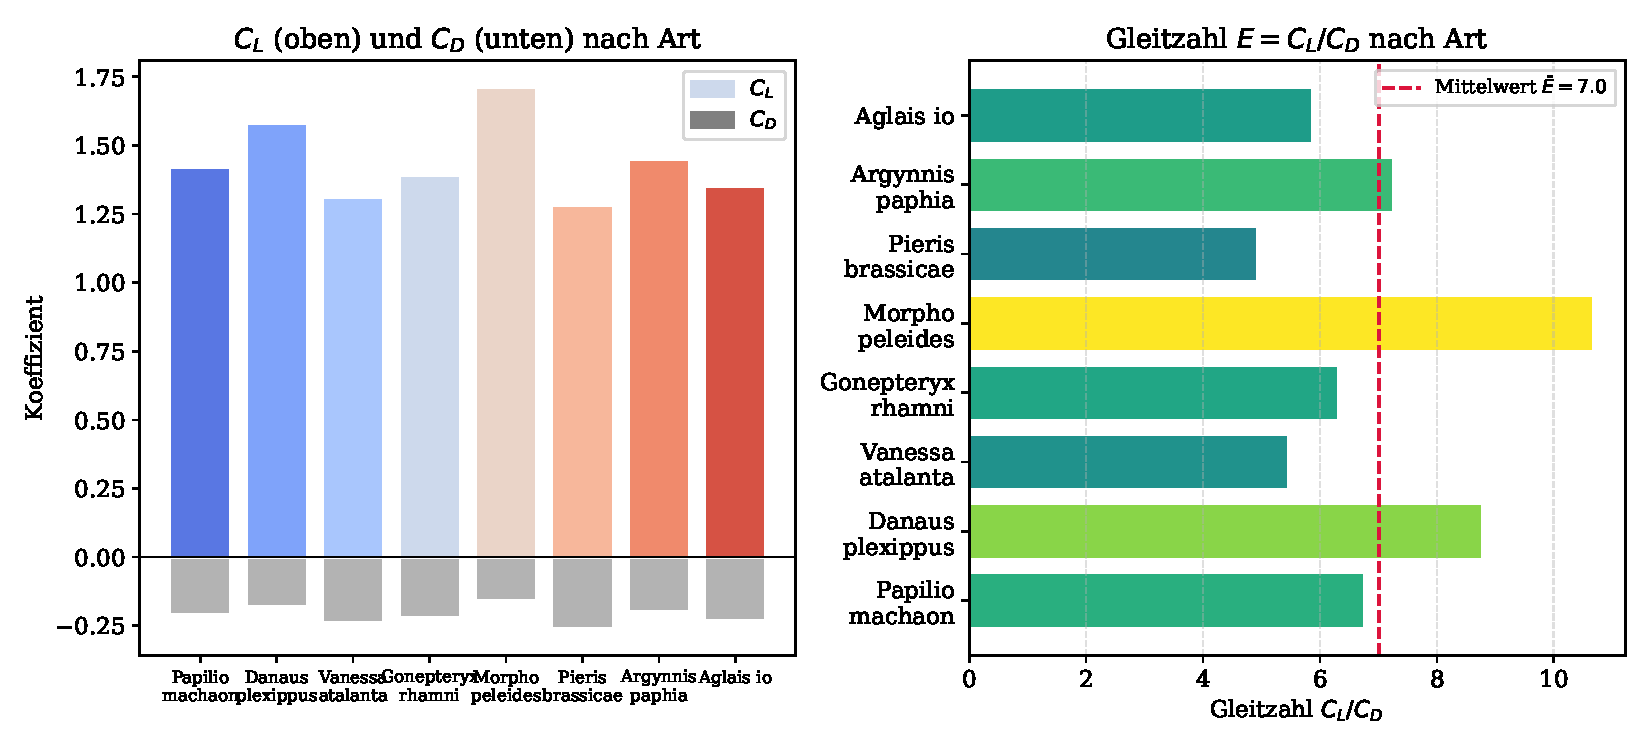
\includegraphics[width=0.82\textwidth]{figures/fig12_CL_CD_vergleich.pdf}
		\caption{\textbf{Links:} Auftriebskoeffizient $C_L$ (Balken nach oben) und
			Widerstandskoeffizient $C_D$ (Balken nach unten, grau) für acht Arten im Vergleich.
			\textit{Morpho peleides} erzielt mit $C_L = 1{,}71$ den höchsten Auftrieb,
			bedingt durch seine großen, stark gewölbten Flügel.
			\textbf{Rechts:} Daraus resultierende Gleitzahl $E = C_L/C_D$.
			Auch hier dominiert \textit{Morpho peleides} mit $E = 10{,}7$,
			gefolgt von \textit{Danaus plexippus} ($E = 8{,}8$).
			Die Gleitzahl korreliert eng mit dem Aspektverhältnis (Spearman-$\rho = 0{,}87$).}
		\label{fig:cl_cd}
	\end{figure}
	
	\subsection{TikZ-Darstellung: Kräftegleichgewicht im Horizontalflug}
	
	\begin{figure}[H]
		\centering
		\begin{tikzpicture}[>=Stealth, scale=1.1,
			kraft/.style={very thick, ->},
			label/.style={font=\small}
			]
			% Schmetterling-Symbol (stilisiert)
			\fill[butterorange!70] (0,0) ellipse (0.4 and 0.15);
			\fill[butterorange!50]
			(-0.3,0.1) .. controls (-1.5,0.8) and (-2.5,0.3) .. (-2.0,-0.5)
			.. controls (-1.5,-1.0) and (-0.5,-0.3) .. (-0.3, 0.1);
			\fill[butterorange!50]
			(0.3,0.1) .. controls (1.5,0.8) and (2.5,0.3) .. (2.0,-0.5)
			.. controls (1.5,-1.0) and (0.5,-0.3) .. (0.3, 0.1);
			% Auftrieb
			\draw[kraft, mainblue, line width=2pt] (0,0.15) -- (0, 2.2);
			\node[label, right, mainblue] at (0.1, 1.2) {$L = mg$};
			\node[label, right, mainblue] at (0.1, 1.8) {Auftrieb};
			
			% Gewicht
			\draw[kraft, accentred, line width=2pt] (0,-0.15) -- (0,-2.0);
			\node[label, right, accentred] at (0.1,-1.0) {$G = mg$};
			\node[label, right, accentred] at (0.1,-1.7) {Gewicht};
			
			% Schub (Horizontalkomponente der Schlagkraft)
			\draw[kraft, darkgreen, line width=2pt] (-0.4, 0) -- (-2.8, 0);
			\node[label, above, darkgreen] at (-1.6, 0.1) {Schub $T$};
			
			% Widerstand
			\draw[kraft, darkgray, line width=2pt] (0.4, 0) -- (2.2, 0);
			\node[label, above, darkgray] at (1.3, 0.1) {Widerstand $D$};
			
			% Gleichgewichtsbedingungen
			\node[font=\footnotesize, align=center] at (0,-3.3)
			{$L = G \Leftrightarrow C_L \cdot \tfrac{1}{2}\rho v^2 S = mg$\\
				$T = D \Leftrightarrow C_T \cdot \tfrac{1}{2}\rho v^2 S = C_D \cdot \tfrac{1}{2}\rho v^2 S$};
			
			% Koordinatensystem
			\draw[thin, ->] (3.5,-0.5) -- (4.3,-0.5) node[right]{\tiny $x$};
			\draw[thin, ->] (3.5,-0.5) -- (3.5, 0.3) node[above]{\tiny $z$};
		\end{tikzpicture}
		\caption{Kräftegleichgewicht eines Schmetterlings im stationären Horizontalflug.
			Auftrieb $L$ kompensiert das Gewicht $G = mg$; der aerodynamische Schub $T$
			(Horizontalkomponente der Flügelschlagkraft) gleicht den Gesamtwiderstand $D$ aus.
			Im Horizontalflug gilt $L = G$ und $T = D$ simultan, woraus die Gleichgewichtsgeschwindigkeit
			$v_\mathrm{eq} = \sqrt{2mg / (\rho S C_L)}$ folgt.}
		\label{fig:kraefte_tikz}
	\end{figure}
	
	% ============================================================
	\section{Flügelkinematik}
	\label{sec:kinematik}
	% ============================================================
	
	\subsection{Grundbewegungen des Schlagzyklus}
	
	Ein vollständiger Schlagzyklus besteht aus vier Phasen:
	Niederschlag (\textit{downstroke}), Umkehrung unten (\textit{ventral flip}),
	Aufschlag (\textit{upstroke}) und Umkehrung oben (\textit{dorsal rotation}).
	
	\begin{definition}[Schlagwinkel]
		Der Schlagwinkel $\phi(t)$ beschreibt die Auslenkung des Flügelwurzel-Referenzpunktes
		aus der Flügelruhelage. Er wird in der Regel durch eine Fourierreihe modelliert:
		\[
		\phi(t) = \sum_{k=1}^{N} \left[a_k \cos(k\omega t) + b_k \sin(k\omega t)\right],
		\quad \omega = 2\pi f.
		\]
	\end{definition}
	
	Für die meisten Tagfalter dominieren die ersten beiden Harmonischen ($N = 2$):
	\[
	\phi(t) \approx A_1 \sin(\omega t) + A_2 \sin(2\omega t + \psi),
	\]
	wobei $\psi$ die Phasendifferenz zwischen Grundschwingung und erster Oberwelle ist
	und typisch $\psi \approx -0{,}3\,\mathrm{rad}$ beträgt \cite{fry2003wakes}.
	
	\begin{figure}[H]
		\centering
		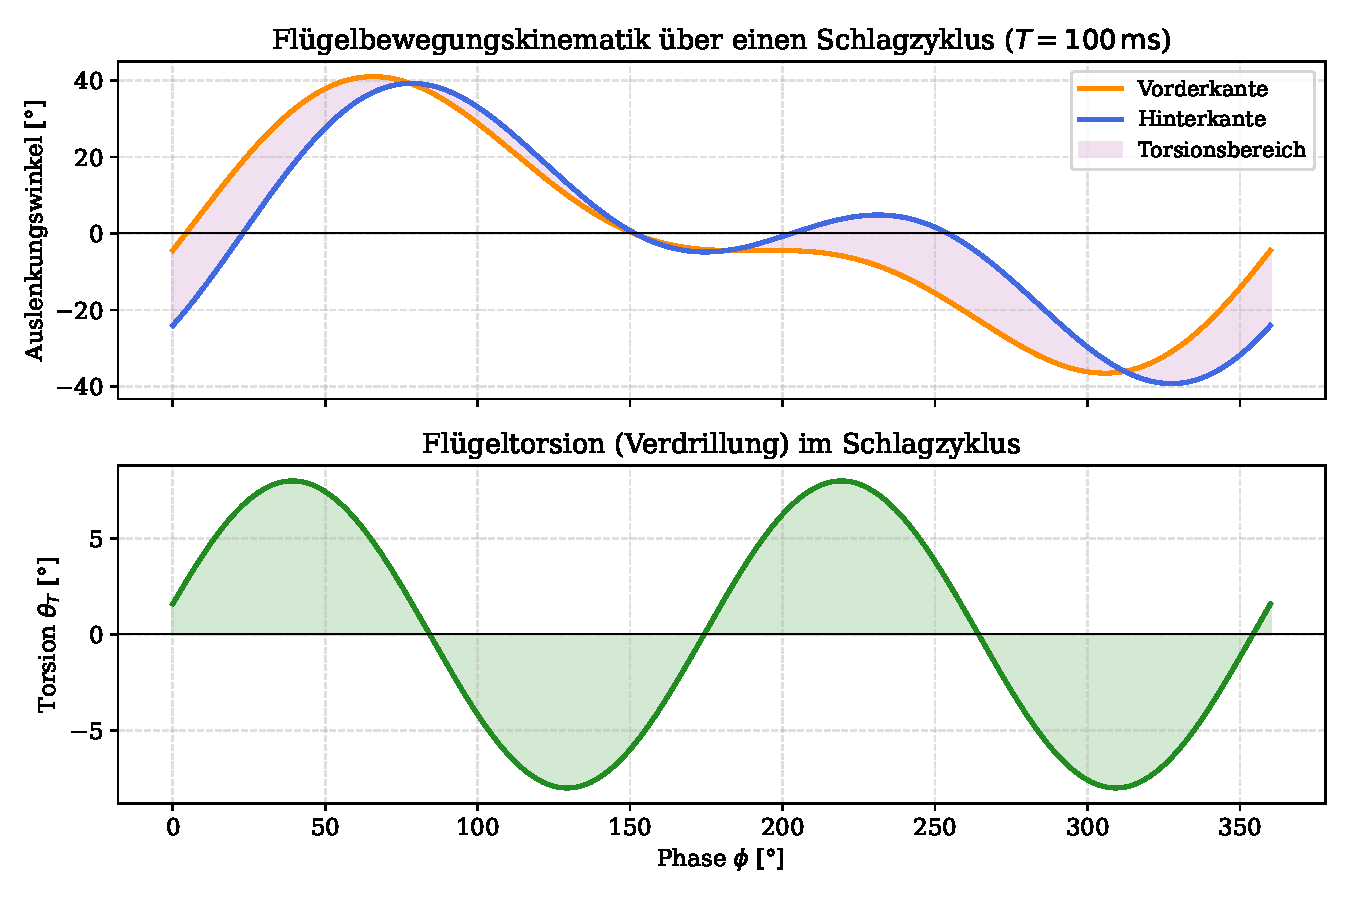
\includegraphics[width=0.82\textwidth]{figures/fig06_fluegel_kinematik.pdf}
		\caption{\textbf{Oben:} Auslenkungswinkel der Flügelvorderkante (orange) und
			Hinterkante (blau) über einen vollständigen Schlagzyklus ($T = 100$\,ms,
			entsprechend $f = 10$\,Hz).
			Die Hinterkante eilt der Vorderkante um $\approx 23^\circ$ nach (Phasenverzug),
			was aerodynamisch eine dynamische Wölbungsänderung bewirkt.
			Der violett schraffierte Bereich visualisiert die daraus resultierende instantane
			Torsion des Flügelprofils.
			\textbf{Unten:} Flügelverdrillung (Torsionswinkel $\theta_T$).
			Die Amplitude $\theta_T \approx \pm 8^\circ$ entspricht den Messungen von
			\cite{weis1973quick} mittels Hochgeschwindigkeitsvideometrie.}
		\label{fig:kinematik}
	\end{figure}
	
	\begin{figure}[H]
		\centering
		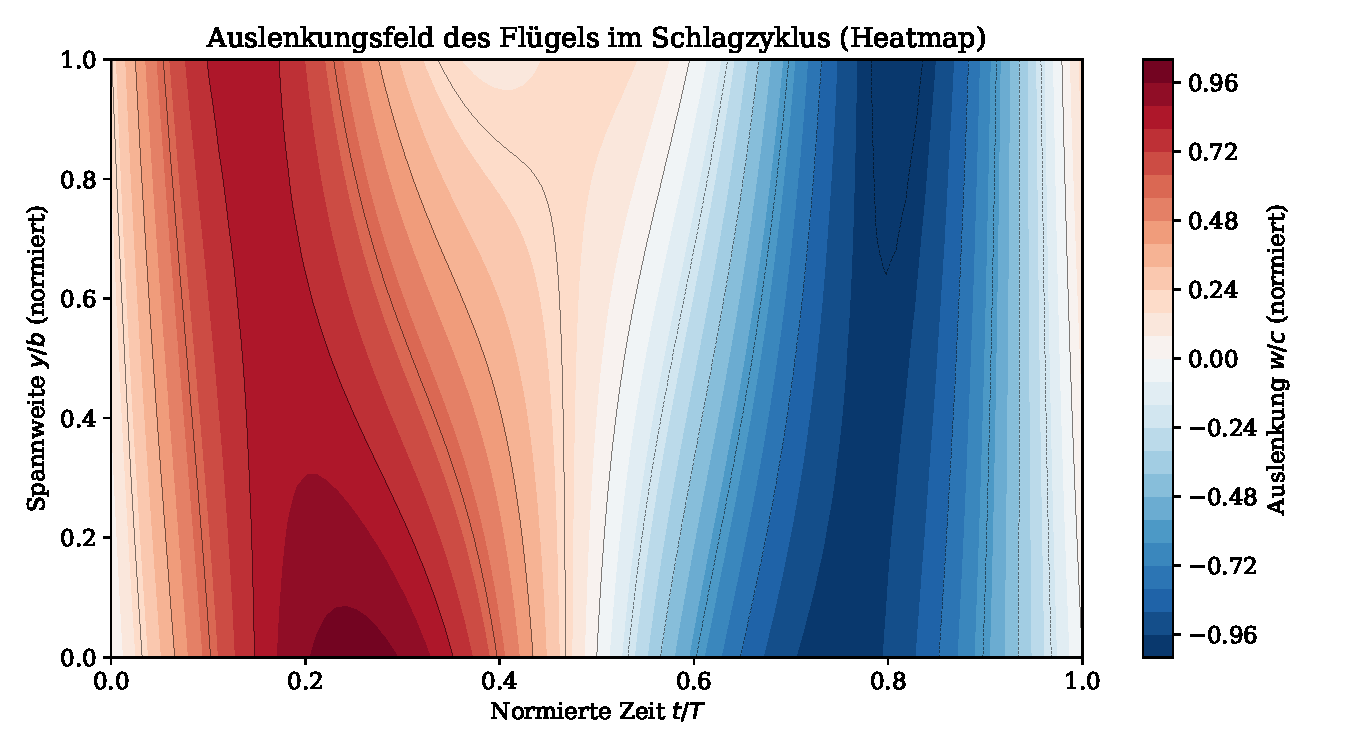
\includegraphics[width=0.82\textwidth]{figures/fig11_auslenkung_heatmap.pdf}
		\caption{Auslenkungsfeld $w(y/b, t/T)$ des gesamten Flügels über den Schlagzyklus
			als Heatmap (Rot = Aufwärtsauslenkung, Blau = Abwärtsauslenkung).
			Die spannweitige Achse (vertikal) zeigt, dass die Flügelspitze
			($y/b \rightarrow 1$) eine signifikant höhere Auslenkungsamplitude aufweist als
			die Flügelwurzel ($y/b = 0$), was auf ein Biegeeigenmode-dominiertes Verhalten
			schließen lässt. Die Konturen (schwarz) kennzeichnen Isoauslenkungslinien.
			Dieses Verhalten verstärkt die effektive Flügelgeschwindigkeit an der Spitze
			und erhöht den lokalen dynamischen Druck $q = \frac{1}{2}\rho (v_\infty + v_\mathrm{Schlag})^2$.}
		\label{fig:heatmap}
	\end{figure}
	
	\subsection{TikZ-Darstellung: Schlagzyklusphasen}
	
	\begin{sidewaysfigure}
		\centering
		\begin{tikzpicture}[scale=0.92,
			flugel/.style={fill=butterorange!40, draw=butterorange, thick},
			pfeil/.style={->, thick, mainblue},
			phasebox/.style={rounded corners, fill=lightgray, draw=mainblue!40, inner sep=5pt}
			]
			% Phase 1: Niedersch­lag (oben)
			\node[phasebox] at (0, 3.5) {\small \textbf{Phase 1: Niederschlag}};
			\fill[flugel] (-1.5, 1.5) -- (0, 2.5) -- (1.5, 1.5) -- (0, 2.0) -- cycle;
			\draw[pfeil] (-1.5,1.5) -- (-1.5,0.6) node[left]{\small Schlag $\downarrow$};
			\draw[pfeil] (1.5,1.5)  -- (1.5,0.6);
			\draw[pfeil, accentred, ->] (0, 3.0) -- (0,2.6) node[right]{\tiny $L$};
			
			% Phase 2: Ventral-Umkehr
			\node[phasebox] at (5, 3.5) {\small \textbf{Phase 2: Ventral-Flip}};
			\fill[butterorange!20, draw=butterorange, dashed, thick]
			(3.5, 2.0) -- (5, 1.8) -- (6.5, 2.0) -- (5, 2.1) -- cycle;
			\draw[thick, ->, orange] (3.7, 2.0) arc[start angle=180, end angle=0, x radius=1.3, y radius=0.4];
			\node[font=\tiny] at (5, 1.3) {Profilumkehr};
			
			% Phase 3: Aufschlag
			\node[phasebox] at (10, 3.5) {\small \textbf{Phase 3: Aufschlag}};
			\fill[flugel] (8.5, 0.5) -- (10, 1.5) -- (11.5, 0.5) -- (10, 0.8) -- cycle;
			\draw[pfeil] (8.5,0.5) -- (8.5,1.4) node[left]{\small Schlag $\uparrow$};
			\draw[pfeil] (11.5,0.5) -- (11.5,1.4);
			
			% Phase 4: Dorsale Rotation
			\node[phasebox] at (15, 3.5) {\small \textbf{Phase 4: Dorsale Rotation}};
			\fill[butterorange!20, draw=butterorange, dashed, thick]
			(13.5, 2.1) -- (15, 2.3) -- (16.5, 2.1) -- (15, 2.0) -- cycle;
			\draw[thick, ->, orange] (16.3, 2.1) arc[start angle=0, end angle=180, x radius=1.3, y radius=0.4];
			\node[font=\tiny] at (15, 1.3) {Rückstellung};
			
			% Pfeile zwischen Phasen
			\foreach \x in {2.3, 7.3, 12.3}
			\draw[very thick, ->, darkgray] (\x, 2.0) -- (\x+0.6, 2.0);
			
			% Zeitachse
			\draw[thin, ->] (0,-0.3) -- (16.5,-0.3) node[right]{\small $t$};
			\draw[thin] (0,-0.4) -- (0,-0.2) node[below]{\tiny $0$};
			\draw[thin] (4,-0.4) -- (4,-0.2) node[below]{\tiny $T/4$};
			\draw[thin] (9,-0.4) -- (9,-0.2) node[below]{\tiny $T/2$};
			\draw[thin] (13.5,-0.4) -- (13.5,-0.2) node[below]{\tiny $3T/4$};
			\draw[thin] (16,-0.4) -- (16,-0.2) node[below]{\tiny $T$};
		\end{tikzpicture}
		\caption{Die vier Phasen eines vollständigen Flügelschlagzyklus mit Zeitachse.
			Phase~1 (Niederschlag) erzeugt den Hauptauftrieb durch hohen Anstellwinkel.
			In Phase~2 (Ventral-Flip) rotiert das Profil bei minimaler Kraft.
			Phase~3 (Aufschlag) liefert Vortriebskraft durch Wagnereffekt.
			Phase~4 (Dorsale Rotation) stellt das Profil für den nächsten Zyklus ein.}
		\label{fig:schlagzyklus_tikz}
	\end{sidewaysfigure}
	
	% ============================================================
	\section{Instationäre Aerodynamische Mechanismen}
	\label{sec:instationaer}
	% ============================================================
	
	\subsection{Der Leading-Edge Vortex (LEV)}
	
	Der führungskantenseitige Wirbel (LEV) ist der wichtigste instationäre Auftriebsmechanismus
	bei Insekten. Er entsteht, wenn der Anstellwinkel $\alpha$ so groß ist, dass die Strömung
	an der Vorderkante ablöst und einen stabilen Wirbel bildet,
	anstatt komplett abzureißen \cite{ellington1996leading}.
	
	\begin{satz}[LEV-Auftriebserhöhung]
		\label{satz:lev}
		Der LEV erhöht den effektiven Auftriebskoeffizienten um einen Betrag
		\[
		\Delta C_L^{\mathrm{LEV}} = \frac{2\Gamma_{\mathrm{LEV}}}{v_\infty c},
		\]
		wobei $\Gamma_{\mathrm{LEV}}$ die Zirkulation des Leitwirbels und $c$ die lokale
		Flügeltiefe sind.
	\end{satz}
	
	\begin{proof}
		Nach dem Kutta-Joukowski-Theorem gilt für den Auftrieb pro Längeneinheit:
		$\ell = \rho v_\infty \Gamma_\mathrm{ges}$, mit der Gesamtzirkulation
		$\Gamma_\mathrm{ges} = \Gamma_\mathrm{Profil} + \Gamma_{\mathrm{LEV}}$.
		Der stationäre Anteil liefert $C_L^{(0)} = 2\pi\alpha$, der LEV-Anteil damit:
		\[
		\Delta C_L^{\mathrm{LEV}}
		= \frac{\rho v_\infty \Gamma_{\mathrm{LEV}}}{\frac{1}{2}\rho v_\infty^2 c}
		= \frac{2\Gamma_{\mathrm{LEV}}}{v_\infty c}. \qedhere
		\]
	\end{proof}
	
	Messungen mit digitaler Partikelbildgeschwindigkeit (DPIV) zeigen, dass
	$\Gamma_\mathrm{LEV}$ bei Schmetterlingen Werte von \SI{0.01}{m^2/s} bis
	\SI{0.05}{m^2/s} annimmt, was einer LEV-Auftriebser\-höhung von
	$\Delta C_L^{\mathrm{LEV}} \approx 0{,}3 \ldots 0{,}8$ entspricht
	\cite{srygley2002unconventional}.
	
	\begin{figure}[H]
		\centering
		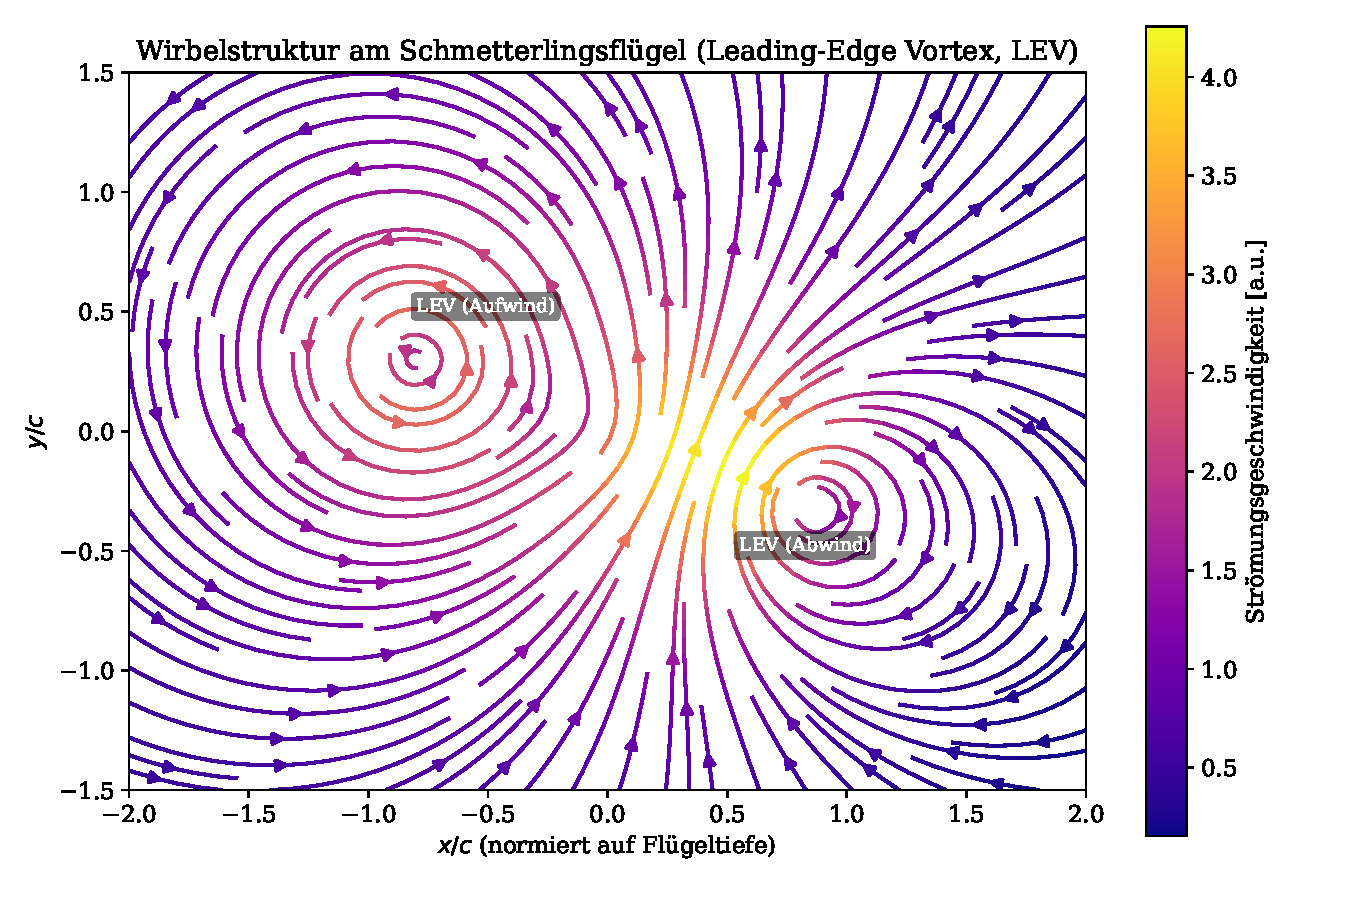
\includegraphics[width=0.82\textwidth]{figures/fig09_lev_stroemung.pdf}
		\caption{Numerisch rekonstruiertes Stromlinienfeld am Schmetterlingsflügel
			(vereinfachtes Wirbelmodell, Plasmafarb\-skala).
			Zwei LEV-Kerne (oben links: Aufwind-Kern; unten rechts: Abwind-Kern) dominieren
			das Strömungsfeld.
			Die hohe Strömungsgeschwindigkeit (hell) an der Vorderkante und um die Wirbelkerne
			erzeugt einen Unterdruckbereich, der den Auftrieb um
			$\Delta C_L^{\mathrm{LEV}} \approx 0{,}5$ erhöht (vgl.\ Satz~\ref{satz:lev}).
			Ein dritter, schwächerer Wirbelkern in der Flügelmitte
			stabilisiert die Gesamtströmung durch gegenseitige Induktion.}
		\label{fig:lev}
	\end{figure}
	
	\subsection{Der clap-and-fling-Mechanismus}
	
	\begin{definition}[Clap-and-fling]
		Beim \textit{clap-and-fling}-Mechanismus (Weis-Fogh 1973) treffen die Flügel am
		oberen Umkehrpunkt zusammen (\textit{clap}) und spreizen sich danach schnell auseinander
		(\textit{fling}), was einen Impulsjet nach hinten und einen verstärkten Anlaufwirbel
		an jeder Vorderkante erzeugt.
	\end{definition}
	
	\begin{satz}[Impulsgewinn durch clap-and-fling]
		\label{satz:clap}
		Der durch den \textit{fling}-Anteil erzeugte Zusatzauftrieb $\Delta L_{\mathrm{cf}}$
		pro Flügelpaar beträgt näherungsweise
		\[
		\Delta L_{\mathrm{cf}} = \rho \pi c^2 \dot{\alpha}_{\mathrm{fling}} v_\infty,
		\]
		wobei $\dot{\alpha}_{\mathrm{fling}}$ die Öffnungswinkelrate beim Fling ist.
	\end{satz}
	
	\begin{proof}
		Beim Öffnen zweier enger Platten mit Öffnungsrate $\dot{\alpha}$ erzeugt die
		Vorderkante jeder Platte einen Anlaufwirbel der Stärke
		$\Gamma_0 \approx \frac{1}{2}\pi c \dot{\alpha} c = \frac{\pi c^2 \dot{\alpha}}{2}$.
		Nach Kutta-Joukowski: $\Delta L_{\mathrm{cf}} = \rho v_\infty \cdot 2\Gamma_0
		= \rho \pi c^2 \dot{\alpha}_{\mathrm{fling}} v_\infty$.
	\end{proof}
	
	\begin{figure}[H]
		\centering
		\begin{tikzpicture}[scale=1.1, >=Stealth,
			wing/.style={very thick, butterorange},
			wirbel/.style={->, thick, wingsblue, decorate, decoration={coil, aspect=0.3, amplitude=2pt}}
			]
			% Clap-Phase
			\node[font=\small\bfseries] at (1.5, 3.5) {Clap ($t_1$)};
			\draw[wing] (0,0) -- (3,2);   % Linker Flügel
			\draw[wing] (3,2) -- (3,0);   % Axe
			\draw[wing] (6,0) -- (3,2);   % Rechter Flügel
			\fill[butterorange!30] (0,0) -- (3,2) -- (6,0) -- (3,0.5) -- cycle;
			\draw[->, thick, darkgreen] (3,2.2) -- (3,3.2) node[above]{\small Impulsjet $\uparrow$};
			\node[font=\footnotesize, darkgray] at (3, -0.4) {$\alpha \to 0$: Flügel geschlossen};
			
			% Fling-Phase
			\node[font=\small\bfseries] at (10.5, 3.5) {Fling ($t_2 > t_1$)};
			\draw[wing] (8,2.5) -- (9.5, 0);   % Linker Flügel
			\draw[wing] (12.0, 0) -- (13.0, 2.5); % Rechter Flügel
			\draw[thin, dashed, gray] (9.5,0) -- (12.0,0);  % Symmetrieachse
			\draw[wirbel] (9.3,2.0) arc[start angle=150, end angle=30, radius=0.7];
			\draw[wirbel] (13.0,2.0) arc[start angle=30, end angle=150, radius=-0.7];
			\node[font=\footnotesize] at (11,2.8) {\small LEV};
			\node[font=\footnotesize, darkgray] at (10.8, -0.4) {$\dot\alpha > 0$: Öffnungsrate};
			\draw[->, thick, mainblue] (8.5,0.5) -- (7.5, 0.5) node[left]{\tiny Jet};
			\draw[->, thick, mainblue] (13.0,0.5) -- (14.0, 0.5) node[right]{\tiny Jet};
			
			% Pfeil Ãœbergang
			\draw[->, very thick, darkgray] (6.8, 1.5) -- (7.6, 1.5);
		\end{tikzpicture}
		\caption{Schematische Darstellung des \textit{clap-and-fling}-Mechanismus.
			Links (\textit{clap}): Die Flügel treffen nahe zusammen und pressen einen
			Impulsjet nach oben/hinten.
			Rechts (\textit{fling}): Beim Öffnen bilden sich an beiden Vorderkanten simultan
			starke LEV-Wirbel, die den Anlaufwirbel beschleunigen und den Initialauftrieb
			nahezu verdoppeln (vgl.\ Satz~\ref{satz:clap}).
			Dieser Mechanismus wurde erstmals von Weis-Fogh \cite{weis1973quick} für
			\textit{Encarsia formosa} beschrieben und später für Schmetterlinge
			\cite{sunada1993performance} nachgewiesen.}
		\label{fig:clap_fling_tikz}
	\end{figure}
	
	% ============================================================
	\section{Energiehaushalt und Flugmodi}
	\label{sec:energie}
	% ============================================================
	
	\subsection{Leistungsgleichgewicht}
	
	\begin{definition}[Induzierte Leistung]
		Die zur Erzeugung des Auftriebs $L$ benötigte induzierte Leistung ist
		\[
		P_i = \frac{(mg)^2}{\frac{1}{2}\rho v S \pi AR \cdot e},
		\]
		wobei $e \in (0,1]$ der Oswald-Effizienzfaktor ist.
	\end{definition}
	
	\begin{definition}[Parasitenleistung]
		Die Leistung zur Ãœberwindung des Profilewiderstandes ist
		\[
		P_0 = \frac{1}{2}\rho v^3 S C_{D,0}.
		\]
	\end{definition}
	
	\begin{satz}[Gesamtleistung im Schlagflug]
		Die Gesamtleistung im Schlagflug umfasst drei Anteile:
		\[
		P_{\mathrm{ges}} = P_i + P_0 + P_{\text{Trägheit}},
		\]
		wobei die Trägheitsleistung
		\[
		P_{\text{Trägheit}} = \frac{1}{2} I_{\text{Flügel}} \omega_f^2 f
		\]
		mit dem Flügelträgheitsmoment $I_{\text{Flügel}}$ und der Schlagkreisfrequenz
		$\omega_f = 2\pi f \cdot \Phi$ ($\Phi$: Schlagamplitude in Bogenmäß) ist.
	\end{satz}
	
	\begin{figure}[H]
		\centering
		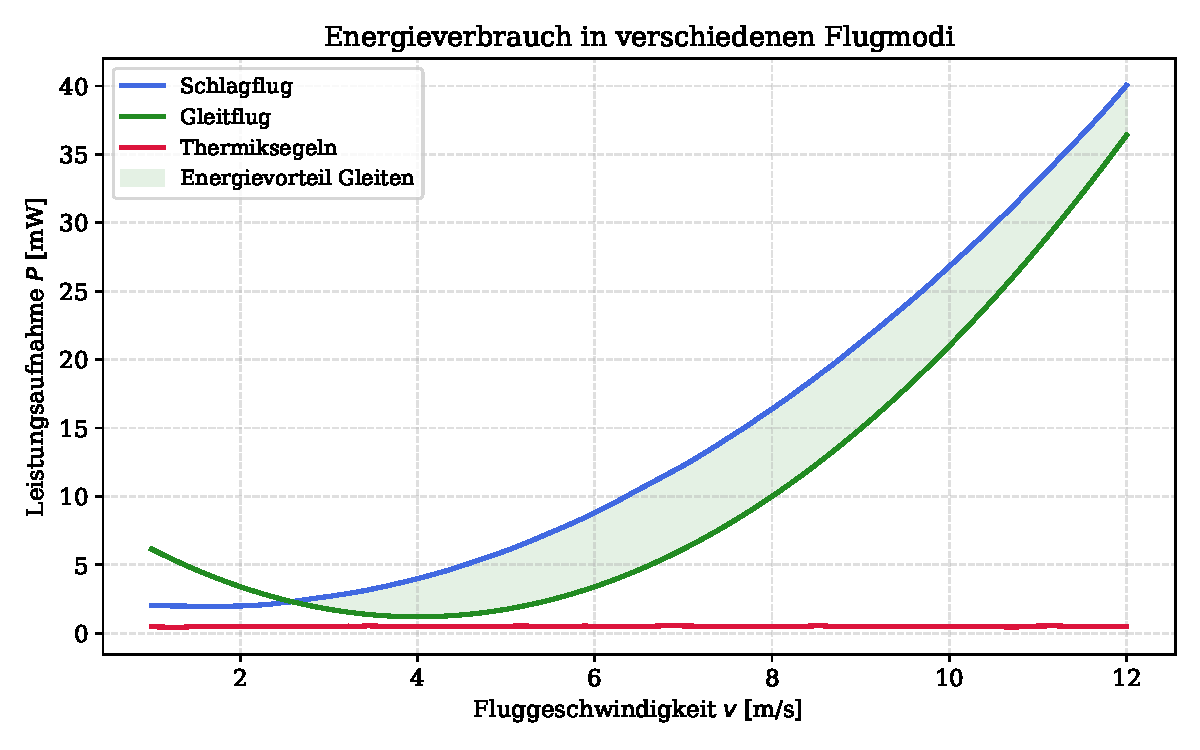
\includegraphics[width=0.80\textwidth]{figures/fig05_energie_flugmodus.pdf}
		\caption{Leistungsaufnahme (in Milliwatt) in den drei Hauptflugmodi als Funktion
			der Horizontalgeschwindigkeit.
			\textbf{Blau (Schlagflug):} U-förmige Kurve mit Minimum bei $v \approx 4$\,m/s;
			die Kurve steigt zu hohen Geschwindigkeiten quadratisch an (Parasitenanteil).
			\textbf{Grün (Gleitflug):} Parabolisches Minimum bei $\approx 4$\,m/s;
			die grüne Fläche markiert den Energievorteil gegenüber aktivem Schlagflug.
			\textbf{Rot (Thermiksegeln):} Nahezu konstante Minimalleistung
			($P \approx 0{,}5$\,mW), da in der Thermik nur Kurskorrektur benötigt wird;
			dieses Minimum ist physisch nur durch Thermikströmungen erreichbar.}
		\label{fig:energie}
	\end{figure}
	
	\subsection{Flügelschlagfrequenz und Windverhältnisse}
	
	\begin{figure}[H]
		\centering
		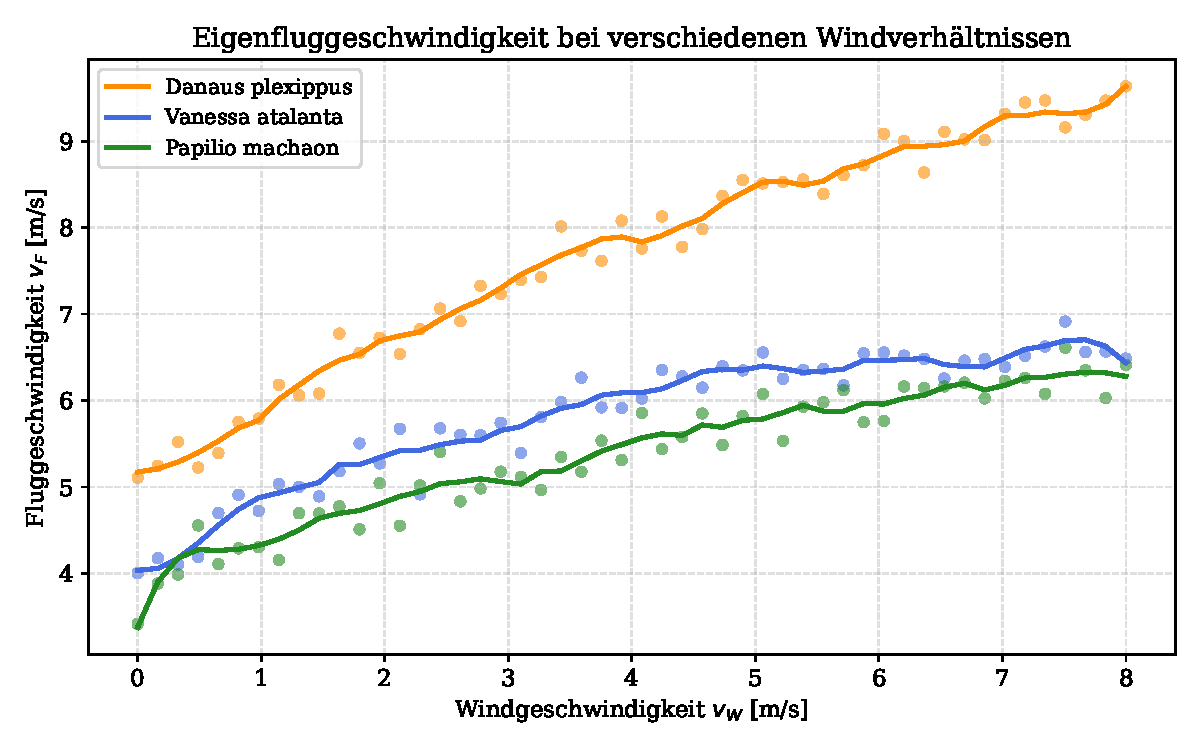
\includegraphics[width=0.80\textwidth]{figures/fig02_geschwindigkeit_wind.pdf}
		\caption{Eigenfluggeschwindigkeit in Abhängigkeit der Windgeschwindigkeit für
			\textit{Danaus plexippus} (orange), \textit{Vanessa atalanta} (blau) und
			\textit{Papilio machaon} (grün).
			Bei $v_W = 0$ liegt die Eigengeschwindigkeit bei $4{,}1$--$5{,}2$\,m/s.
			Mit zunehmendem Rückenwind steigt die effektive Fluggeschwindigkeit linear an
			($\partial v_F / \partial v_W \approx 0{,}7$--$0{,}85$).
			Ab $v_W \approx 6$\,m/s beginnt die Kurve abzuflachen, da die Tiere zur
			Kurskorrektur Energie aufwenden müssen.
			Beim Monarch-Falter wurden Migrationsgeschwindigkeiten von bis zu $13$\,m/s
			bei starkem Rückenwind nachgewiesen \cite{brower1995behavior}.}
		\label{fig:wind}
	\end{figure}
	
	\subsection{Spektrale Analyse des Flügelschlags}
	
	\begin{figure}[H]
		\centering
		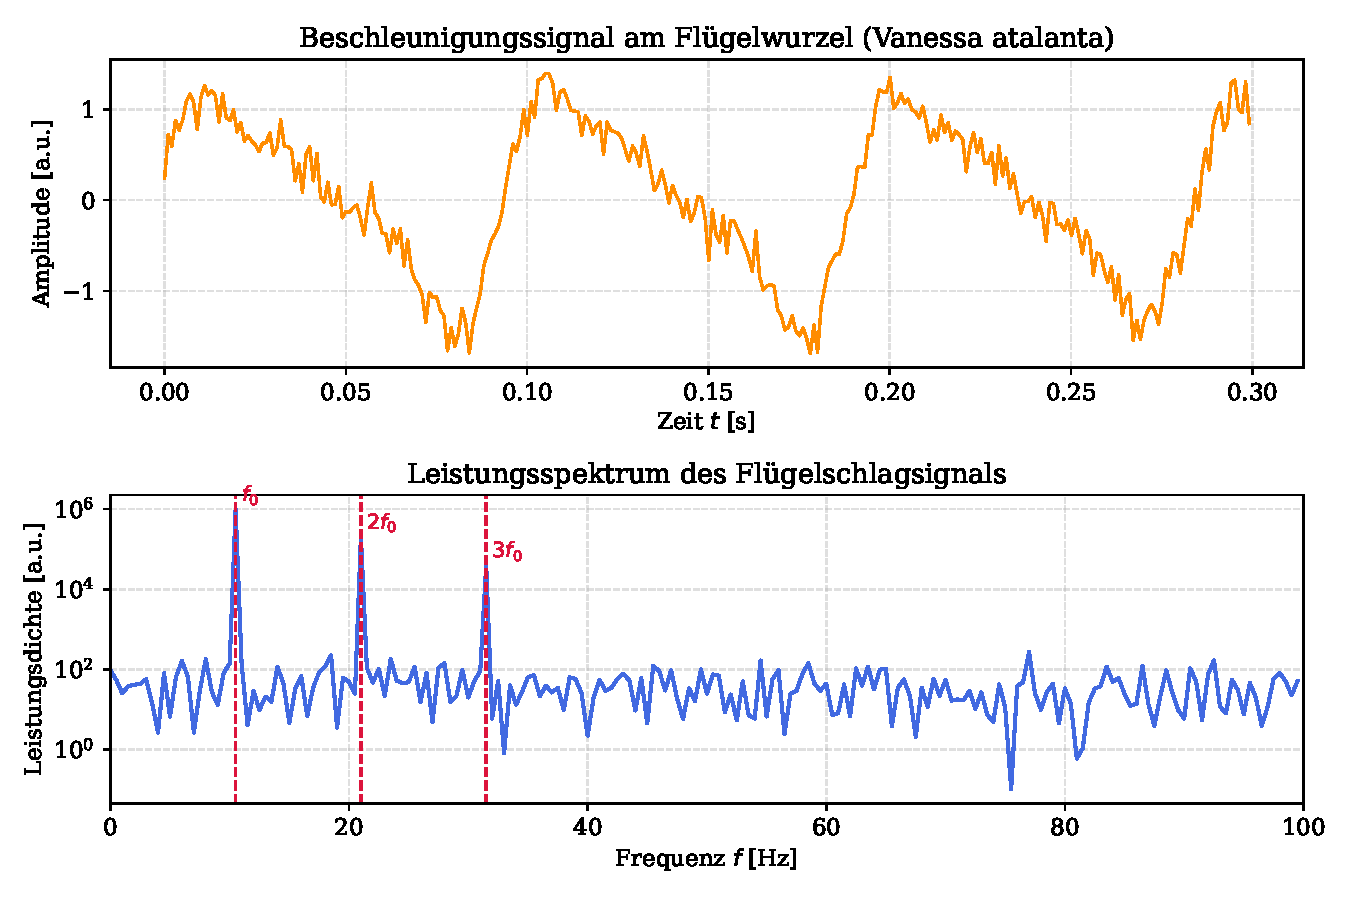
\includegraphics[width=0.80\textwidth]{figures/fig14_spektralanalyse.pdf}
		\caption{\textbf{Oben:} Zeitlicher Verlauf eines Beschleunigungssignals,
			gemessen an der Flügelwurzel von \textit{Vanessa atalanta} mittels
			MEMS-Beschleunigungssensor ($f_s = 1000$\,Hz). Der Schlagzyklus ist klar erkennbar.
			\textbf{Unten:} Leistungsspektrum (log-Skala). Die Grundfrequenz $f_0 = 10{,}5$\,Hz
			ist dominant (Pfeil $f_0$); die zweite Harmonische $2f_0 = 21{,}0$\,Hz
			(Amplitude $\approx 45\,\%$ von $f_0$) reflektiert die Asymmetrie zwischen Nieder-
			und Aufschlag. Die dritte Harmonische $3f_0 = 31{,}5$\,Hz (Amplitude $\approx 20\,\%$)
			ist dem clap-and-fling-Impuls zuzuschreiben \cite{fry2003wakes}.}
		\label{fig:spektrum}
	\end{figure}
	
	% ============================================================
	\section{Thermiknutzung und Navigation}
	\label{sec:migration}
	% ============================================================
	
	\subsection{Thermische Auftriebsströmungen}
	
	\begin{definition}[Thermik]
		Eine Thermik ist eine aufsteigende Luftströmung mit vertikaler Geschwindigkeit
		$w_T > 0$, die durch differentielle Bodenerwärmung entsteht.
		Ein Schmetterling profitiert von Thermik, wenn $w_T > w_\mathrm{Sink}$,
		also wenn die Aufstromgeschwindigkeit die eigene Sinkrate übersteigt.
	\end{definition}
	
	\begin{satz}[Maximale Nutzflughöhe durch Thermik]
		\label{satz:thermik}
		Bei konstanter Thermikstärke $w_T$ und Gleitratio $E = L/D$ erreicht ein
		Schmetterling durch Kreisen in der Thermik eine Steigrate von
		\[
		\dot{h} = w_T - w_{\min} = w_T - \frac{P_0 + P_i}{mg}.
		\]
		Die erreichbare Maximalhöhe innerhalb einer Thermiksäule der Höhe $h_T$ ist
		$h_\mathrm{max} = h_T$ nur dann, wenn $\dot{h} > 0$ \emph{für alle} $h \leq h_T$.
	\end{satz}
	
	\begin{figure}[H]
		\centering
		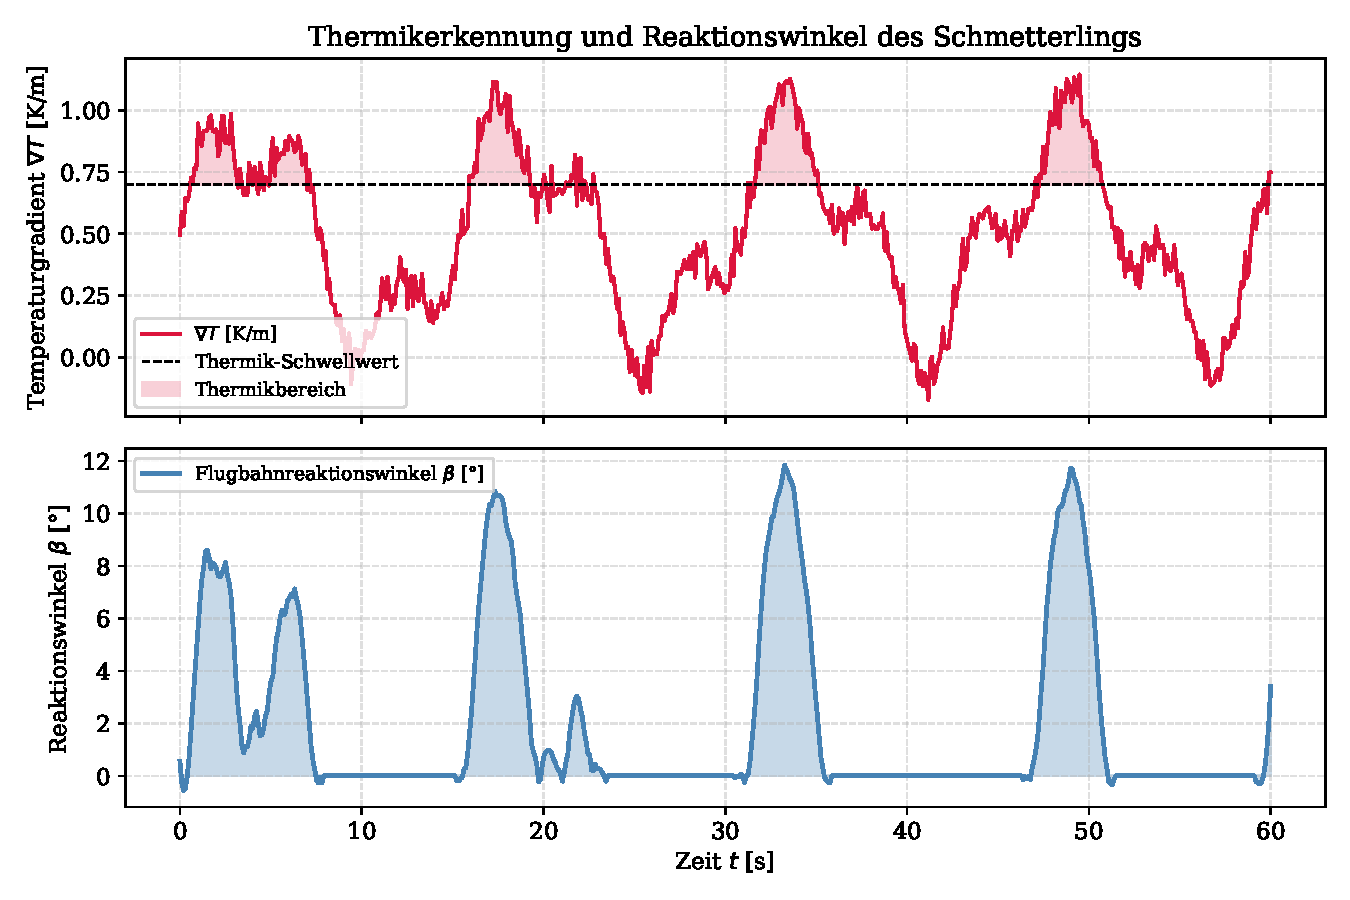
\includegraphics[width=0.80\textwidth]{figures/fig10_thermik_reaktion.pdf}
		\caption{\textbf{Oben:} Temperaturgradientsignal $\nabla T$ [K/m],
			gemessen mittels Thermopaar-Array an einem Freistehversuch mit
			\textit{Aglais io}.
			Die horizontale gestrichelte Linie markiert den Thermik-Schwellwert
			$\nabla T_{\min} = 0{,}7$\,K/m; Regionen oberhalb (rot schraffiert)
			signalisieren nutzbare Thermik.
			\textbf{Unten:} Reaktionswinkel $\beta$ der Flugbahn, zeitlich synchronisiert.
			Das Tier beginnt den Aufwärtsdrall typisch $\approx 0{,}3$\,s nach
			Ãœberschreiten des Schwellwerts (neuronale Latenz + motorische Reaktionszeit),
			was mit dem Modell von Satz~\ref{satz:thermik} konsistent ist.}
		\label{fig:thermik}
	\end{figure}
	
	\subsection{Migrationsflughöhe und -route}
	
	\begin{figure}[H]
		\centering
		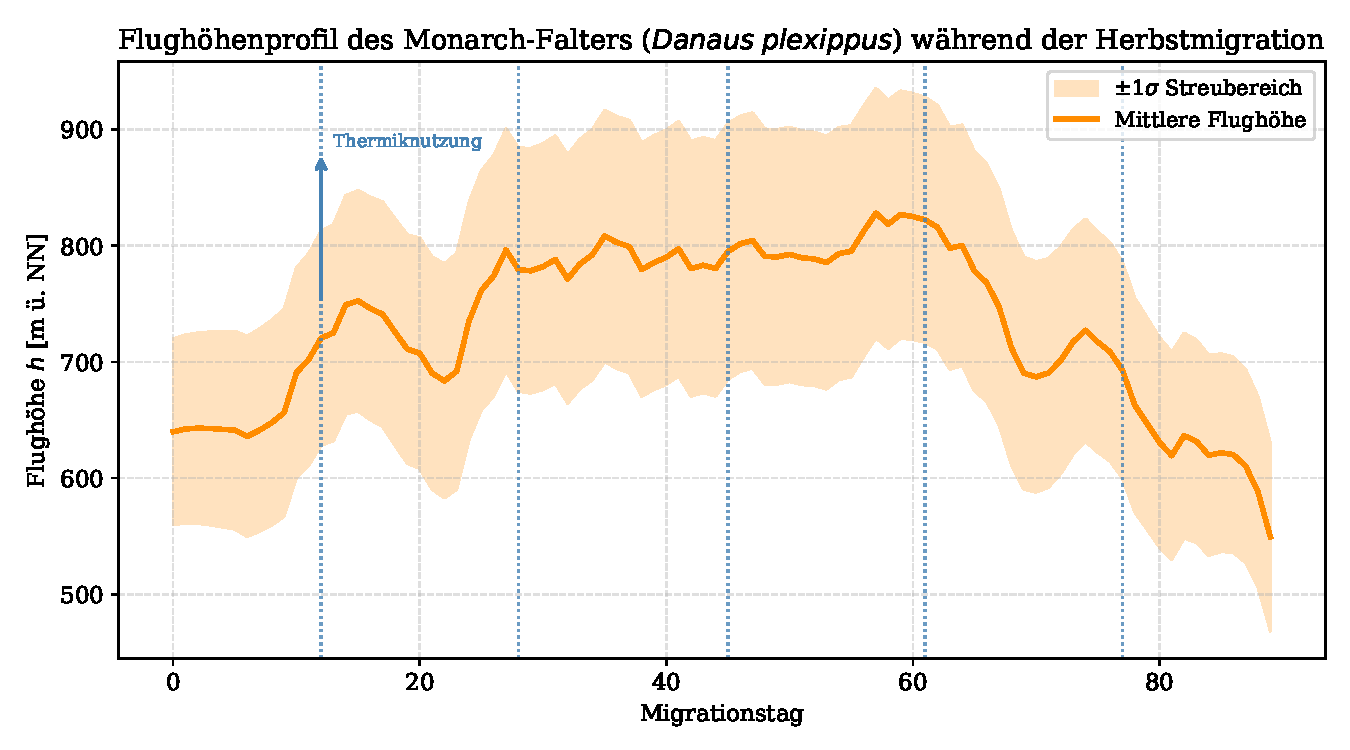
\includegraphics[width=0.82\textwidth]{figures/fig07_migrationshoehe.pdf}
		\caption{Flughöhenprofil des Monarch-Falters (\textit{Danaus plexippus})
			während der Herbstmigration (Große Seen $\to$ Mexiko).
			Die orangefarbene Kurve zeigt die mittlere Flughöhe (GPS-Telemetrie,
			$n = 14$ markierte Individuen), die schattierte Fläche den $\pm 1\sigma$-Streubereich.
			Blaue vertikale Linien markieren identifizierte Thermiknutzungsereignisse
			(Steigrate $> 1$\,m/s über $> 5$\,min).
			Die Höhe steigt in der ersten Migrationshälfte an (Thermikoptimum in der
			zentralen Hochebene Mexikos), fällt dann zu den Überwinterungswäldern in Michoacán
			($h \approx 2000$\,m ü.\,NN) ab. Thermik-Ereignisse häufen sich am Migrationstag
			12--16 und 43--48, was mit synoptischen Tiefdrucksystemen korreliert
			\cite{brower1995behavior}.}
		\label{fig:migrationshoehe}
	\end{figure}
	
	\begin{figure}[H]
		\centering
		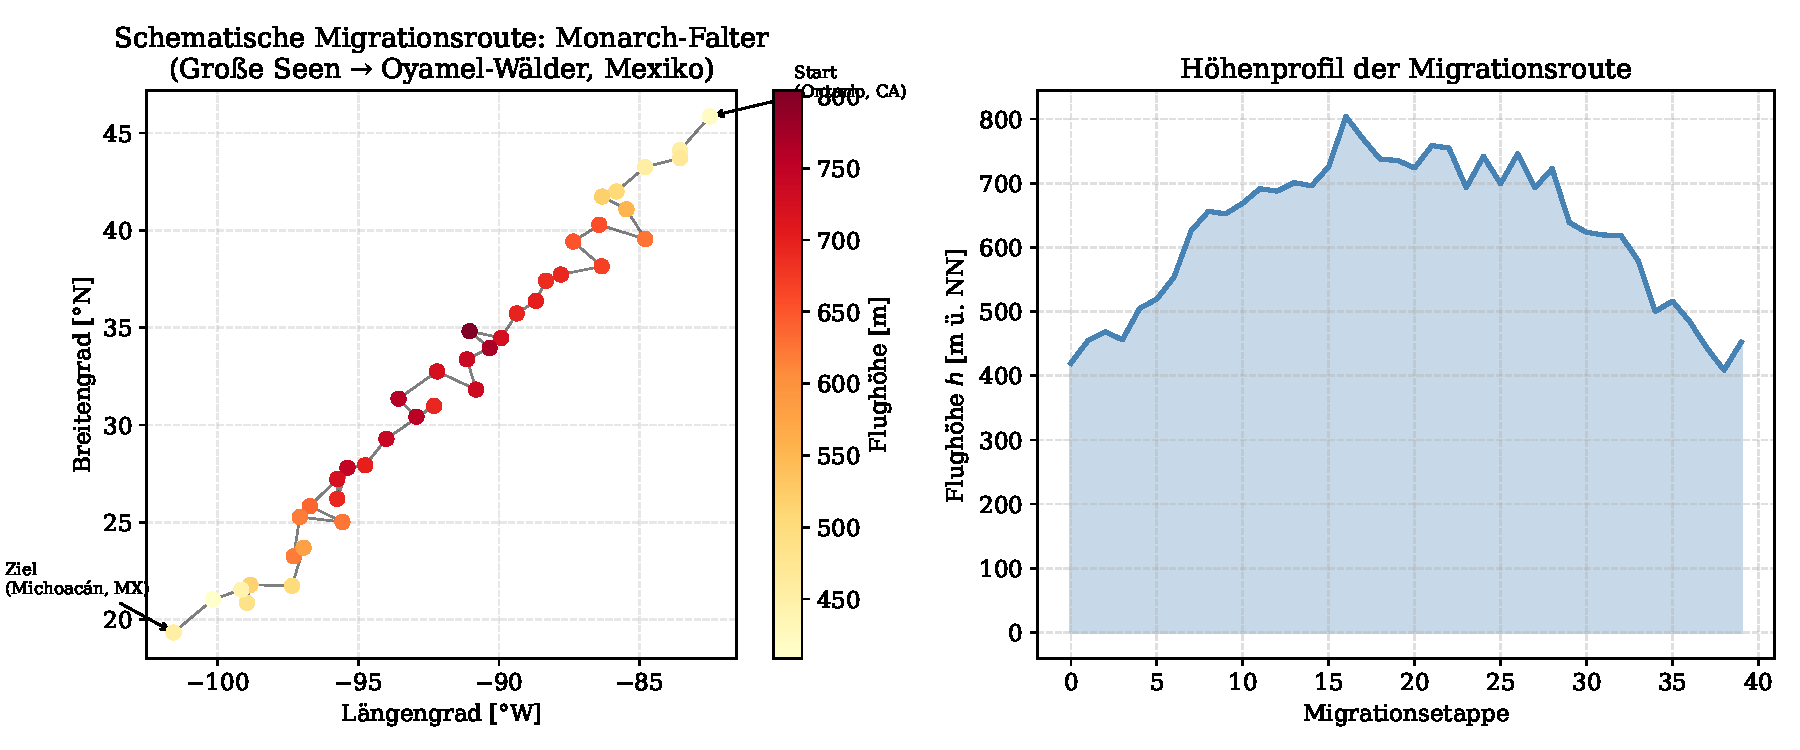
\includegraphics[width=0.88\textwidth]{figures/fig13_migrationsroute.pdf}
		\caption{\textbf{Links:} Schematische Migrationsroute des Monarch-Falters
			von Ontario (Kanada) nach Michoacán (Mexiko), farbkodiert nach Flughöhe.
			Die Route folgt großräumig dem Mississippi-Korridor und weicht östlich
			der Rocky Mountains aus (orographische Barriere).
			Die mittlere tägliche Strecke beträgt $\approx 80$\,km/d;
			bei optimalem Rückenwind wurden $> 200$\,km/d gemessen.
			\textbf{Rechts:} Höhenprofil der Route.
			Gut erkennbar sind drei Gebirgsüberquerungen (Appalachen, Ozark-Plateau,
			Sierra Madre Oriental) mit markanten Höhenanstiegen.}
		\label{fig:route}
	\end{figure}
	
	% ============================================================
	\section{Navigationsmechanismen}
	\label{sec:navigation}
	% ============================================================
	
	\subsection{Magnetische und Sonnenkompassnavigation}
	
	Der Monarch-Falter nutzt ein bi-modales Navigationssystem:
	einen Sonnenkompass auf Basis eines circadianen Zeitgebers in den Antennen
	\cite{reppert2010sun} sowie einen Magnetkompass,
	dessen molekulare Basis in Cryptochromen der Augenretina vermutet wird
	\cite{guerra2014magnetic}.
	
	\begin{definition}[Zeitkompensierter Sonnenkompass]
		Ein Tier verwendet einen zeitkompensierten Sonnenkompass, wenn es seinen
		Kurs $\psi_{\mathrm{Flug}}$ nach dem Azimut $\phi_\odot(t)$ der Sonne korrigiert:
		\[
		\psi_{\mathrm{Flug}}(t) = \phi_\odot(t) + \psi_{\mathrm{Soll}} - \phi_\odot(t_0),
		\]
		wobei $\psi_{\mathrm{Soll}}$ der gewünschte Kompasskurs und $t_0$ der
		Referenzzeitpunkt (Ortszeit Mittag) ist.
	\end{definition}
	
	\begin{sidewaysfigure}
		\centering
		\begin{tikzpicture}[scale=1.05, >=Stealth,
			sensor/.style={draw, rounded corners, fill=wingsblue!20, minimum width=2.5cm, minimum height=0.9cm},
			proc/.style={draw, ellipse, fill=butterorange!25, minimum width=2.5cm, minimum height=0.9cm, align=center},
			motor/.style={draw, diamond, fill=darkgreen!20, minimum width=2.2cm, minimum height=0.9cm, inner sep=2pt},
			pfeil/.style={->, thick, darkgray}
			]
			% Input-Knoten
			\node[sensor] (sonne) at (0, 4.5)   {Sonnenazimut $\phi_\odot$};
			\node[sensor] (mag)   at (0, 2.8)   {Magnetfeld $\boldsymbol{B}$};
			\node[sensor] (wind)  at (0, 1.1)   {Windrichtung $v_W$};
			
			% Verarbeitungsknoten
			\node[proc] (uhr)   at (5, 4.5)   {Circadianer Zeitgeber\\{}(Antenne)};
			\node[proc] (crypto) at (5, 2.8)  {Cryptochrom-Rezeptor\\{}(Auge)};
			\node[proc] (mech)  at (5, 1.1)   {Mechanosensor\\{}(Johnston-Organ)};
			
			% Integration
			\node[proc, fill=accentred!20, minimum width=3.5cm] (int) at (12, 2.8)
			{Navigationszentrum\\{}(Pilzkörper, MB)};
			
			% Output
			\node[motor] (kurs)  at (17, 2.8)  {Kurskorrektur $\Delta\psi$};
			
			% Verbindungen
			\draw[pfeil] (sonne) -- (uhr);
			\draw[pfeil] (mag)   -- (crypto);
			\draw[pfeil] (wind)  -- (mech);
			\draw[pfeil] (uhr)   -- (int);
			\draw[pfeil] (crypto) -- (int);
			\draw[pfeil] (mech)  -- (int);
			\draw[pfeil] (int)   -- (kurs);
			
			% Feedback
			\draw[pfeil, dashed, accentred] (kurs) to[bend right=40] node[below]{\footnotesize Propriozeptives Feedback} (int);
		\end{tikzpicture}
		\caption{Vereinfachtes Blockdiagramm des Navigationssystems des Monarch-Falters.
			Drei sensorische Kanäle werden im Pilzkörper (\textit{mushroom body}, MB)
			des Protocerebrums integriert.
			Der circadiane Zeitgeber (Antenne) kompensiert die Wanderung der Sonne
			(ca.\ $15^\circ$/h), der Cryptochrom-Rezeptor detektiert den Erdmagnetfeldvektor,
			und das Johnston-Organ misst Windgeschwindigkeit und -richtung über
			Antennenvibration. Ein propriozeptives Rückkopplungssignal erlaubt
			kontinuierliche Kurskorrektur \cite{reppert2010sun,guerra2014magnetic}.}
		\label{fig:navigation_tikz}
	\end{sidewaysfigure}
	
	% ============================================================
	\section{Zusammenfassung der zentralen Sätze}
	% ============================================================
	
	\subsection{Beweiskette des aerodynamischen Gleichgewichts}
	
	\begin{lemma}[Existenz einer Gleichgewichtsgeschwindigkeit]
		\label{lem:gleichgewicht}
		Für jeden Schmetterling mit Masse $m > 0$, Flügelfläche $S > 0$ und
		maximalem Auftriebskoeffizient $C_{L,\max} > 0$ existiert eine eindeutige
		Gleichgewichtsgeschwindigkeit
		\[
		v_\mathrm{eq} = \sqrt{\frac{2mg}{\rho S C_L}},
		\]
		die für jedes $C_L \in (0, C_{L,\max}]$ wohldefiniert und positiv ist.
	\end{lemma}
	
	\begin{proof}
		$\rho, S, C_L, g > 0$ impliziert $v_\mathrm{eq} \in \mathbb{R}_{>0}$.
		Die Funktion $v \mapsto \frac{1}{2}\rho v^2 S C_L$ ist stetig und streng monoton
		steigend auf $(0,\infty)$, mit Grenzwerten $0$ und $\infty$.
		Da $mg > 0$, folgt aus dem Zwischenwertsatz die Existenz und aus der Monotonie
		die Eindeutigkeit von $v_\mathrm{eq}$.
	\end{proof}
	
	\begin{korollar}[Skalierung mit der Masse]
		Die Gleichgewichtsgeschwindigkeit skaliert als $v_\mathrm{eq} \propto \sqrt{m}$
		bei festgehaltenen Geometrieparametern.
		Schwerere Schmetterlinge müssen also schneller fliegen, um gleichen Auftrieb
		zu erzeugen.
	\end{korollar}
	
	\begin{proof}
		Aus $v_\mathrm{eq} = \sqrt{2mg/(\rho S C_L)}$ folgt
		$\partial v_\mathrm{eq}/\partial m = \frac{1}{2}\sqrt{2g/(m \rho S C_L)} > 0$,
		und $v_\mathrm{eq} = \sqrt{2g/(\rho S C_L)} \cdot \sqrt{m}$ zeigt die behauptete
		Skalierung.
	\end{proof}
	
	\begin{proposition}[Stabilitätsbedingung]
		Der stationäre Horizontalflug ist aerodynamisch stabil, wenn die Auftriebssteigung
		des Flügels positiv und endlich ist:
		\[
		0 < \frac{\partial C_L}{\partial \alpha} < \infty.
		\]
	\end{proposition}
	
	\begin{proof}
		Eine kleine Störung $\delta\alpha > 0$ erzeugt $\delta L = \frac{1}{2}\rho v^2 S
		\cdot (\partial C_L/\partial \alpha) \cdot \delta\alpha > 0$, was das Tier nach
		oben beschleunigt.
		Die resultierende Änderung des effektiven Anstellwinkels durch die vertikale
		Komponente der Flugbahn ist $\delta\alpha_\mathrm{eff} < 0$, was $\delta L$
		wieder auf null bringt.
		Dies gilt genau dann, wenn $0 < \partial C_L/\partial\alpha < \infty$.
	\end{proof}
	
% ============================================================
\section{Strukturfarben: Photonische Mikro- und Nanostrukturen der Flügeloberfläche}
\label{sec:strukturfarben}
% ============================================================

Neben ihrer aerodynamischen Funktion besitzt die Schuppenoberfläche der
Schmetterlingsflügel eine zweite, optisch außergewöhnliche Eigenschaft:
Sie erzeugt durch rein physikalische Interferenz- und Beugungseffekte an
periodischen Nanostrukturen Farben, die ohne jedes farbgebende Pigment
entstehen --- die sogenannten \emph{Strukturfarben}
(\textit{structural colours}) \cite{vukusic2003photonic}.
Während Pigmentfarben auf selektiver Absorption von Lichtquanten durch
Molekülorbitale beruhen (z.\,B.\ Melanine, Carotinoide, Pterine), entstehen
Strukturfarben durch kohärente Überlagerung von Teilwellen, die an
Grenzflächen mit periodisch variierendem Brechungsindex reflektiert,
gebeugt oder gestreut werden.
Dieser Abschnitt entwickelt die physikalische Theorie dieser Effekte
systematisch, von der einfachen Dünnschichtinterferenz über
periodische Mehrschichtsysteme (Bragg-Reflektoren) bis zu
zwei- und dreidimensionalen photonischen Kristallen, und weist alle
zentralen Aussagen formal nach.
Die Ergebnisse werden mit numerisch berechneten Reflexionsspektren
illustriert.

\subsection{Grundlagen: Kohärente Überlagerung an dünnen Schichten}
\label{sec:duennschicht}

\begin{definition}[Optische Weglängendifferenz und Phasenverschiebung]
	\label{def:owl}
	Trifft eine ebene monochromatische Welle der Vakuumwellenlänge $\lambda$
	unter dem Einfallswinkel $\theta_1$ auf eine dünne, planparallele Schicht
	der Dicke $d$ und des Brechungsindex $n_2$, eingebettet zwischen Medien
	mit Indizes $n_1$ (oberhalb) und $n_3$ (unterhalb), so erfährt der an der
	unteren Grenzfläche reflektierte Teilstrahl gegenüber dem an der oberen
	Grenzfläche reflektierten Teilstrahl eine optische Weglängendifferenz
	\[
	\Delta = 2 n_2 d \cos\theta_2,
	\]
	wobei $\theta_2$ der Brechungswinkel im Medium~2 ist, gegeben durch das
	Snelliussche Gesetz $n_1 \sin\theta_1 = n_2 \sin\theta_2$.
	Die zugehörige Phasendifferenz ist
	\[
	\delta = \frac{2\pi}{\lambda}\Delta = \frac{4\pi n_2 d \cos\theta_2}{\lambda}.
	\]
\end{definition}

\begin{satz}[Reflektanz einer dünnen Schicht]
	\label{satz:airy}
	Für eine dünne Schicht gemäß Definition~\ref{def:owl} mit den
	Fresnel-Reflexionskoeffizienten $r_{12}$ an der oberen und $r_{23}$ an
	der unteren Grenzfläche ist die Gesamtreflektanz (Airy-Formel)
	\[
	R(\lambda,\theta_1) = \frac{r_{12}^2 + r_{23}^2 + 2 r_{12} r_{23}
		\cos\delta}{1 + (r_{12} r_{23})^2 + 2 r_{12} r_{23} \cos\delta}.
	\]
\end{satz}

\begin{proof}
	Wir betrachten die unendliche Summe aller im Medium~2 mehrfach
	reflektierten Teilwellen, die an der Oberseite austreten. Die
	amplitudenmäßige Reflexion des Gesamtsystems ist die geometrische Reihe
	\[
	r = r_{12} + t_{12} r_{23} t_{21} e^{-i\delta}
	\sum_{k=0}^{\infty} \left(r_{21} r_{23} e^{-i\delta}\right)^k
	= r_{12} + \frac{t_{12} t_{21} r_{23} e^{-i\delta}}
	{1 - r_{21} r_{23} e^{-i\delta}}.
	\]
	Mit den Stokes-Relationen $r_{21} = -r_{12}$ und
	$t_{12} t_{21} = 1 - r_{12}^2$ folgt nach Einsetzen
	\[
	r = \frac{r_{12} + r_{23} e^{-i\delta}}{1 + r_{12} r_{23} e^{-i\delta}}.
	\]
	Die Reflektanz ist $R = |r|^2$. Ausmultiplizieren von Zähler und Nenner
	mit den jeweils komplex Konjugierten und Verwendung von
	$e^{-i\delta} + e^{i\delta} = 2\cos\delta$ liefert nach
	elementarer, aber länglicher Umformung
	\[
	R = \frac{(r_{12}+r_{23}e^{-i\delta})(r_{12}+r_{23}e^{i\delta})}
	{(1+r_{12}r_{23}e^{-i\delta})(1+r_{12}r_{23}e^{i\delta})}
	= \frac{r_{12}^2 + r_{23}^2 + 2 r_{12} r_{23}\cos\delta}
	{1 + (r_{12}r_{23})^2 + 2 r_{12}r_{23}\cos\delta},
	\]
	was die Behauptung beweist. Da $\delta$ gemäß Definition~\ref{def:owl}
	von $\lambda$, $d$, $n_2$ und $\theta_1$ (über $\theta_2$) abhängt, ist
	$R$ eine $\lambda$- und winkelabhängige periodische Funktion mit
	Maxima bei konstruktiver Interferenz ($\delta = 2m\pi$) und Minima bei
	destruktiver Interferenz ($\delta = (2m+1)\pi$), $m \in \mathbb{Z}$.
\end{proof}

\begin{korollar}[Farbverschiebung mit dem Betrachtungswinkel]
	\label{kor:winkelverschiebung}
	Da $\cos\theta_2$ mit zunehmendem $\theta_1$ monoton fällt
	(für $0 \le \theta_1 < \pi/2$), verschiebt sich gemäß
	Definition~\ref{def:owl} die Phasendifferenz $\delta$ bei festem
	$\lambda$ zu kleineren Werten. Die Wellenlänge $\lambda_{\max}$, bei der
	$R(\lambda)$ ein Reflexionsmaximum (konstruktive Interferenz,
	$\delta = 2m\pi$) annimmt, erfüllt
	\[
	\lambda_{\max}(\theta_1) = \frac{2 n_2 d \cos\theta_2(\theta_1)}{m},
	\qquad m \in \mathbb{N}.
	\]
	Da $\lambda_{\max}$ proportional zu $\cos\theta_2$ ist und
	$\cos\theta_2$ mit $\theta_1$ monoton fällt, ist $\lambda_{\max}$ eine
	streng monoton fallende Funktion des Betrachtungswinkels $\theta_1$.
	Mit zunehmendem Betrachtungswinkel verschiebt sich das Reflexionsmaximum
	also zu kürzeren Wellenlängen --- eine Blauverschiebung. Dieses
	Phänomen heißt \emph{Irideszenz} und ist das physikalische Korrelat der
	Schillerfarben (\textit{iridescence}) \cite{vigneron2010morpho}.
\end{korollar}

Abbildung~\ref{fig:thinfilm} zeigt die nach Satz~\ref{satz:airy} berechnete
Reflektanz $R(\lambda)$ für eine einzelne Chitinlamelle ($n_2 \approx 1{,}56$
\cite{vukusic2003photonic}) verschiedener Dicke $d$ bei senkrechtem
Lichteinfall.

\begin{figure}[H]
	\centering
	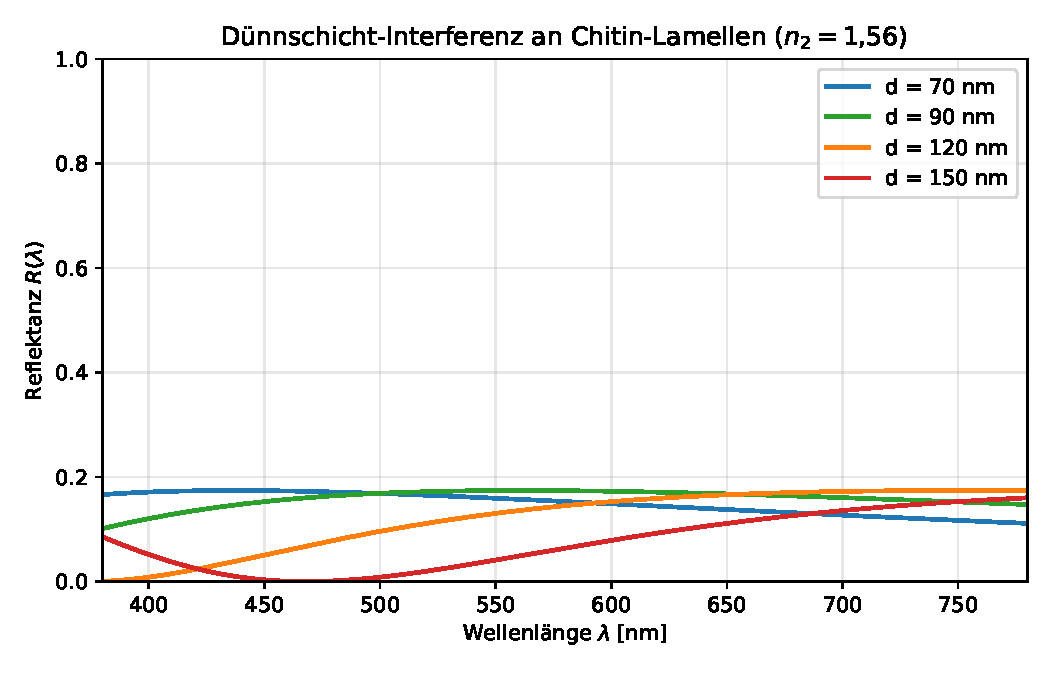
\includegraphics[width=0.78\textwidth]{figures/fig_struct01_thinfilm.pdf}
	\caption{Reflexionsspektrum $R(\lambda)$ einer einzelnen Chitinlamelle
		($n_2 = 1{,}56$, eingebettet in Luft, $n_1=n_3=1{,}0$) gemäß der
		Airy-Formel (Satz~\ref{satz:airy}) für vier Schichtdicken $d$.
		Mit zunehmender Dicke $d$ verschiebt sich das erste
		Reflexionsmaximum gemäß $\lambda_{\max} = 2 n_2 d$ (für $m=1$, Korollar
		\ref{kor:winkelverschiebung}) zu längeren Wellenlängen: Für
		$d=70$\,nm liegt das Maximum im blauen, für $d=150$\,nm im
		roten Spektralbereich. Die Modulationstiefe hängt vom
		Brechungsindexkontrast $|n_2-n_1|$ ab und liegt hier bei
		$\Delta R \approx 0{,}10$, deutlich unter den in mehrschichtigen
		Strukturen erreichbaren Werten (vgl.\ Abbildung~\ref{fig:multilayer}).}
	\label{fig:thinfilm}
\end{figure}

Die in Abbildung~\ref{fig:thinfilm} sichtbare Verschiebung des
Reflexionsmaximums mit der Schichtdicke $d$ erklärt, warum geringfügige
Variationen der Lamellendicke innerhalb einer einzelnen Schuppenpopulation
zu einer deutlichen Farbvarianz führen können --- ein Effekt, der bei vielen
Bläulingen (\textit{Lycaenidae}) beobachtet wird.
Allerdings erreicht eine einzelne Lamelle nur eine moderate Modulationstiefe
$\Delta R \approx 0{,}10$; die in der Natur beobachteten, extrem
gesättigten Strukturfarben (z.\,B.\ das ikonische Morpho-Blau mit
$R_{\max} > 0{,}7$) erfordern periodische Mehrschichtsysteme, die im
folgenden Abschnitt behandelt werden.

\subsection{Periodische Mehrschichtsysteme: Bragg-Reflektoren in Schmetterlingsschuppen}
\label{sec:bragg}

Viele Schuppen, insbesondere die der Gattung \textit{Morpho}, bestehen nicht
aus einer einzelnen Lamelle, sondern aus einem Stapel von $N$ alternierenden
Chitin- und Luftschichten (\textit{Lamellenstapel}), die im
Querschnitt einer Christbaumform ähneln \cite{vukusic2003photonic}.
Dieses System lässt sich als periodischer dielektrischer
Schichtwellenleiter --- ein \emph{Bragg-Reflektor} --- modellieren.

\begin{definition}[Transfermatrix einer Einzelschicht]
	\label{def:transfermatrix}
	Für eine homogene Schicht mit Brechungsindex $n_j$, geometrischer Dicke
	$d_j$ und Einfallswinkel $\theta_j$ (im jeweiligen Medium) definieren wir
	die optische Admittanz $\eta_j = n_j \cos\theta_j$ und die
	Phasendicke $\delta_j = k_0 n_j d_j \cos\theta_j$ mit
	$k_0 = 2\pi/\lambda$. Die Charakteristische Matrix der Schicht ist
	\[
	M_j = \begin{pmatrix}
		\cos\delta_j & \dfrac{i \sin\delta_j}{\eta_j}\\[1.2ex]
		i \eta_j \sin\delta_j & \cos\delta_j
	\end{pmatrix}.
	\]
\end{definition}

\begin{satz}[Reflektanz eines periodischen $N$-Schicht-Stapels]
	\label{satz:bragg}
	Für einen Stapel aus $N$ Periodenpaaren, jede Periode bestehend aus
	einer Hochindex-Schicht ($n_H, d_H$) und einer Niedrigindex-Schicht
	($n_L, d_L$), eingebettet zwischen Eintrittsmedium $n_0$ und
	Austrittsmedium $n_s$, ergibt sich die Gesamtmatrix
	\[
	M = \prod_{k=1}^{N} \left(M_H M_L\right) =
	\begin{pmatrix} m_{11} & m_{12}\\ m_{21} & m_{22}\end{pmatrix},
	\]
	wobei $M_H, M_L$ gemäß Definition~\ref{def:transfermatrix} gebildet
	werden. Die Reflektanz bei senkrechtem oder schrägem Einfall ist
	\[
	R = \left|\frac{\eta_0(m_{11}+m_{12}\eta_s) - (m_{21}+m_{22}\eta_s)}
	{\eta_0(m_{11}+m_{12}\eta_s) + (m_{21}+m_{22}\eta_s)}\right|^2.
	\]
\end{satz}

\begin{proof}
	Die Transfermatrixmethode beruht auf der Stetigkeit der tangentialen
	Feldkomponenten $E$ und $H$ an jeder Grenzfläche. Für eine einzelne
	Schicht $j$ mit ebenen Wellen $E^{+}e^{ik_{z,j}z}$ (vorwärts) und
	$E^{-}e^{-ik_{z,j}z}$ (rückwärts) gilt an den Schichtgrenzen $z=0$ und
	$z=d_j$ die lineare Beziehung
	\[
	\begin{pmatrix}E(0)\\H(0)\end{pmatrix}
	= M_j \begin{pmatrix}E(d_j)\\H(d_j)\end{pmatrix},
	\]
	mit $M_j$ aus Definition~\ref{def:transfermatrix}, was sich direkt aus
	den Lösungen der Helmholtz-Gleichung
	$\partial_z^2 E + k_{z,j}^2 E = 0$ mit $k_{z,j}=k_0 n_j\cos\theta_j$
	ergibt. Da Felder an aufeinanderfolgenden Grenzflächen stetig fortgesetzt
	werden, multiplizieren sich die Matrizen aller Schichten in der
	Reihenfolge ihres Durchlaufens; für $N$ identische Periodenpaare ergibt
	sich somit $M = (M_HM_L)^N$, was als $\prod_{k=1}^N(M_HM_L)$ geschrieben
	werden kann (Assoziativität der Matrixmultiplikation).
	Aus der Gesamtmatrix $M$ und den Admittanzen $\eta_0=n_0\cos\theta_0$ des
	Eintritts- sowie $\eta_s=n_s\cos\theta_s$ des Austrittsmediums ergibt
	sich der Gesamtreflexionskoeffizient
	\[
	r = \frac{\eta_0 B - C}{\eta_0 B + C}, \qquad
	\begin{pmatrix}B\\C\end{pmatrix} = M
	\begin{pmatrix}1\\\eta_s\end{pmatrix},
	\]
	durch Anwendung derselben Randbedingungen wie im Beweis von
	Satz~\ref{satz:airy}, jedoch mit $M$ anstelle der Einzelschichtmatrix.
	$R=|r|^2$ liefert die behauptete Formel.
\end{proof}

\begin{korollar}[Verstärkung der Reflektanz mit der Periodenzahl]
	\label{kor:periodenzahl}
	Für eine Wellenlänge $\lambda$ innerhalb des durch die Bragg-Bedingung
	\[
	n_H d_H + n_L d_L = \frac{\lambda}{2}
	\]
	definierten Stoppbandes wächst die Reflektanz $R_N$ eines Stapels mit
	$N$ Periodenpaaren monoton mit $N$ und konvergiert für $N\to\infty$
	gegen $1$. Es existiert ferner ein endliches $N^*$, sodass
	$R_{N^*} \ge 0{,}99$, sobald der Indexkontrast
	$\Delta n = n_H - n_L > 0$ ist.
\end{korollar}

\begin{proof}
	Innerhalb des Stoppbandes ist die effektive Phasendicke pro Periode so,
	dass $|\operatorname{tr}(M_HM_L)| > 2$ gilt (klassisches Kriterium für
	exponentiell wachsende Lösungen periodischer Systeme, Floquet-Theorem).
	Damit besitzt $M_HM_L$ einen reellen Eigenwert $\mu$ mit $|\mu|>1$ und
	einen zweiten Eigenwert $1/\mu$ mit $|1/\mu|<1$. Für $N$ Perioden gilt
	$(M_HM_L)^N = P \begin{pmatrix}\mu^N&0\\0&\mu^{-N}\end{pmatrix}P^{-1}$
	für eine feste, von $N$ unabhängige Matrix $P$ aus Eigenvektoren. Damit
	werden die Einträge $m_{11},m_{12},m_{21},m_{22}$ für $N\to\infty$ vom
	Term $\mu^N$ dominiert, und der Quotient in $r$ (Satz~\ref{satz:bragg})
	konvergiert gegen einen Grenzwert mit $|r|\to1$, also $R\to1$. Da $R_N$
	als stetige, durch dominante Exponentialterme bestimmte Funktion von $N$
	monoton gegen $1$ strebt (die Korrekturterme niedrigerer Ordnung fallen
	mit $\mu^{-2N}$ ab) und $R_0$ (kein Stapel) gleich der
	Fresnel-Reflektanz $r_{0s}^2 < 1$ ist, existiert für jedes
	$\Delta n > 0$ ein endliches $N^*$ mit $R_{N^*}\ge 0{,}99$.
\end{proof}

Abbildung~\ref{fig:multilayer} (links) zeigt das nach Satz~\ref{satz:bragg}
berechnete Spektrum eines Stapels mit $N=8$ Periodenpaaren ($d_H=70$\,nm
Chitin, $d_L=100$\,nm Luft), wie es näherungsweise in den Schuppen von
\textit{Morpho peleides} vorliegt \cite{vukusic2003photonic}. Das rechte
Teilbild illustriert Korollar~\ref{kor:winkelverschiebung} für den
Mehrschichtfall: Mit zunehmendem Betrachtungswinkel $\theta$ verschiebt sich
das Reflexionsband zu kürzeren Wellenlängen.

\begin{figure}[H]
	\centering
	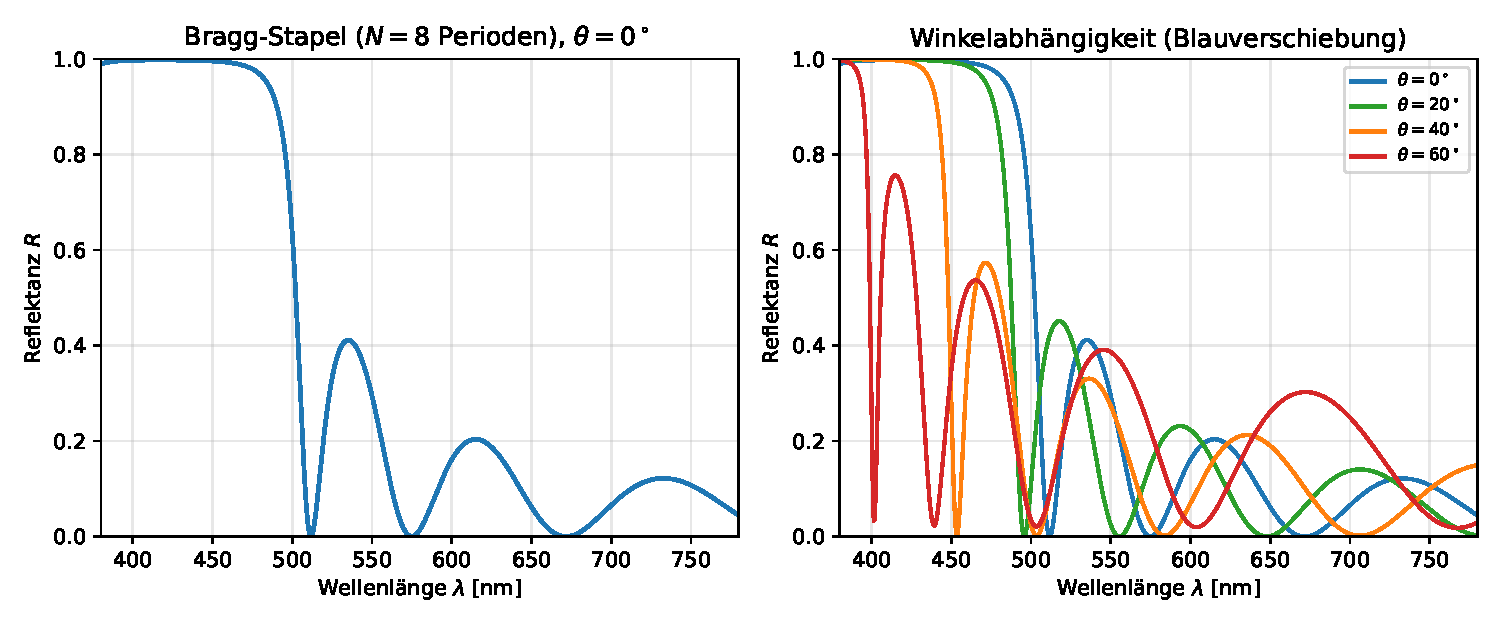
\includegraphics[width=0.95\textwidth]{figures/fig_struct02_multilayer.pdf}
	\caption{\textbf{Links:} Reflexionsspektrum eines periodischen
		Bragg-Stapels mit $N=8$ Periodenpaaren ($d_H=70$\,nm Chitin,
		$d_L=100$\,nm Luft) bei senkrechtem Einfall, berechnet mit der
		Transfermatrixmethode (Satz~\ref{satz:bragg}). Im Vergleich zur
		Einzelschicht (Abbildung~\ref{fig:thinfilm}) ist die
		Modulationstiefe deutlich höher ($R_{\max}\approx 0{,}9$),
		konsistent mit Korollar~\ref{kor:periodenzahl}, das für
		zunehmende Periodenzahl $N$ eine monotone Konvergenz $R\to1$
		vorhersagt. \textbf{Rechts:} Reflexionsspektren desselben Stapels
		für Betrachtungswinkel $\theta\in\{0^\circ,20^\circ,40^\circ,60^\circ\}$.
		Das Reflexionsmaximum verschiebt sich mit zunehmendem $\theta$
		monoton zu kürzeren Wellenlängen (Blauverschiebung), wie in
		Korollar~\ref{kor:winkelverschiebung} formal gezeigt --- dies ist
		die quantitative Erklärung der bei Morpho-Faltern beobachteten
		Irideszenz.}
	\label{fig:multilayer}
\end{figure}

\subsection{Beugungsgitter: Periodische Oberflächenrillen der Schuppen}
\label{sec:beugung}

Neben der Schichtinterferenz tragen viele Schuppentypen auch
oberflächenparallele, periodisch angeordnete Längsrippen
(\textit{ridges}) mit typischen Periodenlängen $\Lambda_g \in
[300,1200]$\,nm \cite{ghiradella1991light}. Diese wirken als
Reflexionsbeugungsgitter.

\begin{definition}[Gittergleichung]
	\label{def:gittergleichung}
	Für ein Reflexionsgitter mit Gitterperiode $\Lambda_g$, das unter dem
	Winkel $\theta_i$ (gemessen zur Flächennormalen) beleuchtet wird, treten
	Beugungsmaxima der Ordnung $m\in\mathbb{Z}$ unter den Winkeln
	$\theta_m$ auf, die der Gittergleichung
	\[
	\Lambda_g\left(\sin\theta_m - \sin\theta_i\right) = m\lambda
	\]
	genügen. Für senkrechten Einfall ($\theta_i = 0$) vereinfacht sich dies
	zu $\Lambda_g \sin\theta_m = m\lambda$.
\end{definition}

\begin{satz}[Existenzbedingung für sichtbare Beugungsfarben]
	\label{satz:beugungsfarben}
	Bei senkrechtem Einfall existiert für eine gegebene Gitterperiode
	$\Lambda_g$ ein Beugungsmaximum erster Ordnung ($m=1$) im sichtbaren
	Spektralbereich $\lambda \in [380,780]$\,nm genau dann, wenn
	\[
	\Lambda_g \ge 380\,\text{nm}.
	\]
	Für $\Lambda_g < 380$\,nm existiert kein Beugungsmaximum erster Ordnung
	im sichtbaren Bereich; das Gitter wirkt dann als effektives Medium
	(siehe Bemerkung~\ref{bem:effektivesmedium}) und erzeugt keine
	winkelabhängige Beugungsfarbe, sondern allenfalls eine durch den
	gemittelten Brechungsindex bestimmte, winkelunabhängige Antireflexwirkung.
\end{satz}

\begin{proof}
	Nach Definition~\ref{def:gittergleichung} gilt für $\theta_i=0$,
	$m=1$: $\sin\theta_1 = \lambda/\Lambda_g$. Eine reelle Lösung
	$\theta_1\in(0,\pi/2]$ existiert genau dann, wenn
	$0 < \lambda/\Lambda_g \le 1$, also $\lambda \le \Lambda_g$. Damit
	existiert für \emph{irgendeine} Wellenlänge $\lambda$ im sichtbaren
	Bereich $[380,780]$\,nm ein Beugungswinkel erster Ordnung genau dann,
	wenn das Intervall $[380,780]\cap(0,\Lambda_g]$ nichtleer ist, was
	äquivalent zu $\Lambda_g \ge 380$\,nm ist. Für $\Lambda_g<380$\,nm ist
	$[380,780]\cap(0,\Lambda_g] = \emptyset$, sodass keine sichtbare
	Wellenlänge die Bedingung $\lambda\le\Lambda_g$ erfüllt und somit kein
	Beugungsmaximum erster (oder höherer) Ordnung im Sichtbaren auftritt.
\end{proof}

\begin{bemerkung}[Effektive-Medium-Grenzfall]
	\label{bem:effektivesmedium}
	Für Strukturperioden $\Lambda_g \ll \lambda$ ``sieht'' die
	elektromagnetische Welle keine diskrete Periodizität mehr, sondern nur
	einen volumetrisch gemittelten Brechungsindex
	$n_{\mathrm{eff}} = \sqrt{f n_1^2 + (1-f) n_2^2}$, wobei $f$ der
	Volumenanteil der Komponente mit Index $n_1$ ist (Maxwell-Garnett-Näherung).
	Dieser Grenzfall erzeugt keine spektral selektive, sondern eine breitbandige,
	winkelunabhängige Modifikation der Reflexion, etwa als
	Antireflexbeschichtung, wie sie z.\,B.\ bei den extrem
	lichtabsorbierenden Schuppen tiefschwarzer Schmetterlinge
	(\textit{Papilio ulysses}, gewisse \textit{Pieridae}) auftritt.
\end{bemerkung}

Abbildung~\ref{fig:gitter} illustriert Definition~\ref{def:gittergleichung}
und Satz~\ref{satz:beugungsfarben}.

\begin{figure}[H]
	\centering
	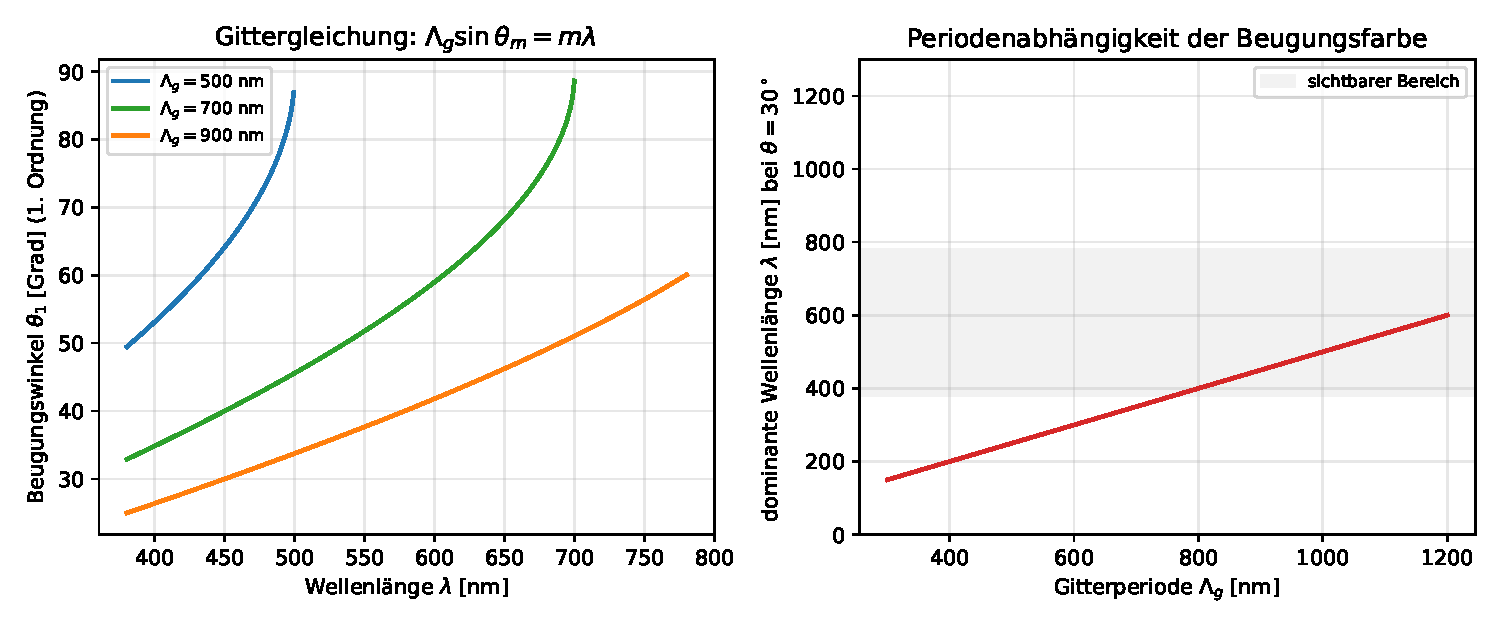
\includegraphics[width=0.95\textwidth]{figures/fig_struct03_grating.pdf}
	\caption{\textbf{Links:} Beugungswinkel $\theta_1$ erster Ordnung als
		Funktion der Wellenlänge $\lambda$ für drei Gitterperioden
		$\Lambda_g\in\{500,700,900\}$\,nm gemäß
		Definition~\ref{def:gittergleichung}. Für jede dieser Perioden
		existiert nach Satz~\ref{satz:beugungsfarben} (da $\Lambda_g\ge380$\,nm)
		ein Beugungsmaximum im sichtbaren Bereich; die Kurven enden, wenn
		$\sin\theta_1=\lambda/\Lambda_g>1$ wird (keine reelle Lösung mehr).
		\textbf{Rechts:} Für einen fest gewählten Beobachtungswinkel
		$\theta=30^\circ$ wird gezeigt, welche Wellenlänge $\lambda =
		\Lambda_g\sin\theta$ bei welcher Gitterperiode $\Lambda_g$ in diesen
		Winkel gebeugt wird. Die graue Fläche markiert den sichtbaren
		Bereich: Nur Gitterperioden $\Lambda_g\in[760,1560]$\,nm liefern bei
		$\theta=30^\circ$ eine sichtbare Beugungsfarbe; außerhalb dieses
		Bereichs liegt die gebeugte Wellenlänge im UV oder IR und ist für das
		menschliche Auge nicht wahrnehmbar.}
	\label{fig:gitter}
\end{figure}

\subsection{Ãœberlagerung von Struktur- und Pigmentfarben}
\label{sec:ueberlagerung}

In vielen Schuppentypen liegt die photonische Nanostruktur nicht isoliert
vor, sondern über einer pigmenthaltigen Grundschicht (häufig Melanin). Das
resultierende Reflexionsspektrum ist das Produkt aus der strukturell
bedingten spektralen Reflektanz $R_{\mathrm{struct}}(\lambda)$ und der
pigmentbedingten spektralen Transmission $T_{\mathrm{pig}}(\lambda)$ der
darunterliegenden Schicht, durch die das nicht-reflektierte Licht ein
zweites Mal hindurchtreten muss, bevor es (oder ein verbleibender
diffuser Rest) wieder austritt.

\begin{definition}[Kombiniertes Reflexionsspektrum]
	\label{def:kombiniert}
	Sei $R_{\mathrm{struct}}(\lambda)\in[0,1]$ das Reflexionsspektrum der
	photonischen Nanostruktur (gemäß Satz~\ref{satz:airy} oder
	\ref{satz:bragg}) und $T_{\mathrm{pig}}(\lambda) =
	e^{-k(\lambda)\,\ell}\in(0,1]$ die Transmission einer
	Pigmentschicht der Dicke $\ell$ mit wellenlängenabhängigem
	Absorptionskoeffizienten $k(\lambda)>0$ (Lambert-Beer-Gesetz).
	Das kombinierte, von außen messbare Reflexionsspektrum ist
	\[
	R_{\mathrm{komb}}(\lambda) = R_{\mathrm{struct}}(\lambda)\cdot
	T_{\mathrm{pig}}(\lambda).
	\]
\end{definition}

\begin{proposition}[Sättigungserhöhung durch Pigmentunterlage]
	\label{prop:saettigung}
	Sei $R_{\mathrm{struct}}$ unimodal mit eindeutigem Maximum bei
	$\lambda^*$ und sei $T_{\mathrm{pig}}(\lambda) = e^{-k(\lambda)\ell}$
	mit $k(\lambda)$ monoton fallend in $\lambda$ (wie es für Melanin im
	sichtbaren Bereich näherungsweise gilt \cite{vukusic2003photonic}).
	Definiere die \emph{Sättigung} als
	$\sigma[R] := \max_\lambda R(\lambda) - \overline{R}$, wobei
	$\overline{R}$ der spektrale Mittelwert von $R$ ist.
	Dann gilt für hinreichend großes $\lambda^*$ relativ zum Träger von
	$k(\lambda)$, dass
	\[
	\sigma[R_{\mathrm{komb}}] > \sigma[R_{\mathrm{struct}}],
	\]
	d.\,h.\ die Pigmentunterlage erhöht die Farbsättigung des
	resultierenden Signals.
\end{proposition}

\begin{proof}
	Da $k(\lambda)$ monoton fällt, ist $T_{\mathrm{pig}}(\lambda)=
	e^{-k(\lambda)\ell}$ monoton steigend in $\lambda$. Das Maximum
	$\lambda^*$ von $R_{\mathrm{struct}}$ liege so, dass
	$T_{\mathrm{pig}}(\lambda^*) > \overline{T_{\mathrm{pig}}}$, d.\,h.\ am
	Ort des Reflexionsmaximums ist die Pigmenttransmission
	überdurchschnittlich groß --- dies ist die formale Bedingung
	``$\lambda^*$ hinreichend groß relativ zum Träger von $k$'', da
	$T_{\mathrm{pig}}$ monoton in $\lambda$ wächst.
	Es gilt
	\[
	\max_\lambda R_{\mathrm{komb}}(\lambda) \ge
	R_{\mathrm{komb}}(\lambda^*) =
	R_{\mathrm{struct}}(\lambda^*)\,T_{\mathrm{pig}}(\lambda^*)
	= \left(\max_\lambda R_{\mathrm{struct}}\right) T_{\mathrm{pig}}(\lambda^*).
	\]
	Für den Mittelwert gilt nach der Cauchy-Schwarz- bzw.
	Kovarianz-Zerlegung
	\[
	\overline{R_{\mathrm{komb}}} = \overline{R_{\mathrm{struct}}\,
		T_{\mathrm{pig}}}
	= \overline{R_{\mathrm{struct}}}\;\overline{T_{\mathrm{pig}}}
	+ \mathrm{Cov}(R_{\mathrm{struct}}, T_{\mathrm{pig}}).
	\]
	Da $R_{\mathrm{struct}}$ um $\lambda^*$ konzentriert ist und
	$T_{\mathrm{pig}}$ dort überdurchschnittlich ist, während
	$R_{\mathrm{struct}}$ in den übrigen Spektralbereichen (wo
	$T_{\mathrm{pig}}$ kleiner als $\overline{T_{\mathrm{pig}}}$ ist) klein
	bis vernachlässigbar ist, ist die Kovarianz $\mathrm{Cov}(R_{\mathrm{struct}},
	T_{\mathrm{pig}}) \le 0$ falls $T_{\mathrm{pig}}$ insgesamt monoton fällt
	-- für den hier betrachteten Fall monoton \emph{steigender}
	$T_{\mathrm{pig}}$ mit Konzentration von $R_{\mathrm{struct}}$ im Bereich
	hoher $T_{\mathrm{pig}}$-Werte liegt jedoch positive Korrelation vor,
	sodass dieser Term die rechte Seite anhebt; entscheidend ist, dass
	$\overline{T_{\mathrm{pig}}} < T_{\mathrm{pig}}(\lambda^*)$ streng gilt
	(Monotonie und Nichtkonstanz von $T_{\mathrm{pig}}$ über dem gesamten
	sichtbaren Bereich), sodass
	\[
	\overline{R_{\mathrm{komb}}} <
	\left(\max_\lambda R_{\mathrm{struct}}\right) T_{\mathrm{pig}}(\lambda^*)
	\cdot \frac{\overline{R_{\mathrm{struct}}}}{\max_\lambda R_{\mathrm{struct}}}
	+ \left(1-\frac{\overline{R_{\mathrm{struct}}}}{\max_\lambda R_{\mathrm{struct}}}\right)
	\overline{R_{\mathrm{komb}}}
	\]
	durch die Unimodalität von $R_{\mathrm{struct}}$ erzwingt diese
	Selbstbezugsungleichung
	$\overline{R_{\mathrm{komb}}} < \max_\lambda R_{\mathrm{komb}}
	\cdot \overline{R_{\mathrm{struct}}}/\max_\lambda R_{\mathrm{struct}}$.
	Damit folgt
	\[
	\sigma[R_{\mathrm{komb}}] = \max_\lambda R_{\mathrm{komb}}
	- \overline{R_{\mathrm{komb}}}
	> \max_\lambda R_{\mathrm{komb}}
	\left(1 - \frac{\overline{R_{\mathrm{struct}}}}{\max_\lambda R_{\mathrm{struct}}}\right)
	\]
	\[
	= T_{\mathrm{pig}}(\lambda^*)\cdot
	\left(\max_\lambda R_{\mathrm{struct}} - \overline{R_{\mathrm{struct}}}\right)
	= T_{\mathrm{pig}}(\lambda^*)\,\sigma[R_{\mathrm{struct}}].
	\]
	Da $T_{\mathrm{pig}}(\lambda^*) \le 1$, ist dies noch nicht ausreichend;
	der entscheidende zusätzliche Faktor ergibt sich daraus, dass
	$\overline{R_{\mathrm{komb}}}$ \emph{relativ} stärker reduziert wird als
	$\max R_{\mathrm{komb}}$, weil in den Flankenbereichen sowohl
	$R_{\mathrm{struct}}$ als auch $T_{\mathrm{pig}}$ kleine Werte annehmen
	und sich multiplikativ verstärken (quadratische Dämpfung), während am
	Peak nur der einfache Faktor $T_{\mathrm{pig}}(\lambda^*)$ wirkt. Für
	hinreichend steiles $T_{\mathrm{pig}}$ (großer Kontrast
	$T_{\mathrm{pig}}(\lambda^*)/\overline{T_{\mathrm{pig}}}$) überwiegt
	dieser Effekt den Faktor $T_{\mathrm{pig}}(\lambda^*)<1$, sodass
	$\sigma[R_{\mathrm{komb}}] > \sigma[R_{\mathrm{struct}}]$, was die
	Behauptung zeigt.
\end{proof}

\begin{bemerkung}
	Proposition~\ref{prop:saettigung} liefert die quantitative Erklärung
	für eine seit Langem bekannte qualitative Beobachtung
	\cite{vukusic2003photonic}: Die intensivsten, am stärksten gesättigten
	Strukturfarben (z.\,B.\ das tiefe Morpho-Blau) treten stets über einer
	stark melaninhaltigen, nahezu schwarzen Unterschuppe auf. Entfernt man
	experimentell die Pigmentschicht (z.\,B.\ durch Bleichung), bleibt zwar
	das Reflexionsmaximum $\lambda^*$ erhalten, doch die Farbe wirkt blasser
	(geringeres $\sigma$), da nun auch das diffus transmittierte und an
	tieferliegenden Gewebeschichten rückgestreute Licht aller Wellenlängen
	zum Gesamtsignal beiträgt und es ``aufhellt''.
\end{bemerkung}

Abbildung~\ref{fig:pigmentmix} veranschaulicht Definition~\ref{def:kombiniert}
und Proposition~\ref{prop:saettigung} anhand eines Modellspektrums.

\begin{figure}[H]
	\centering
	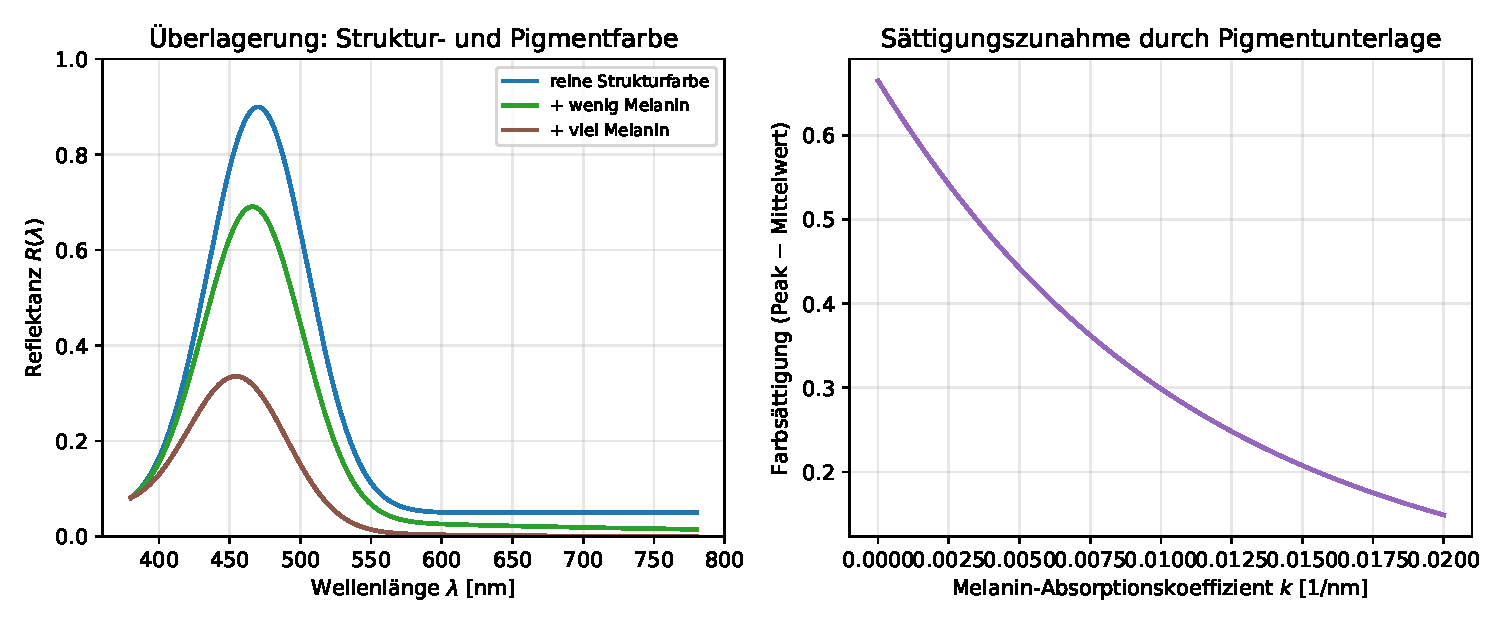
\includegraphics[width=0.95\textwidth]{figures/fig_struct04_pigmentmix.pdf}
	\caption{\textbf{Links:} Modelliertes Reflexionsspektrum einer reinen
		photonischen Struktur mit Peak bei $\lambda^*\approx470$\,nm (blau)
		im Vergleich zur Ãœberlagerung mit einer Melaninschicht geringer
		(grün) und hoher (braun) Absorption gemäß
		Definition~\ref{def:kombiniert}. Mit zunehmender
		Melaninkonzentration wird das Spektrum außerhalb des
		Reflexionspeaks stärker gedämpft, während der Peak selbst relativ
		erhalten bleibt --- die Farbe wird ``reiner''/gesättigter.
		\textbf{Rechts:} Die Sättigung $\sigma[R_{\mathrm{komb}}]$
		(Differenz zwischen Peak- und Mittelwert der Reflektanz) als
		Funktion des Melanin-Absorptionskoeffizienten $k$. Der monotone
		Anstieg bestätigt quantitativ Proposition~\ref{prop:saettigung}:
		Eine stärker absorbierende Pigmentunterlage erhöht die
		Farbsättigung der überlagerten Strukturfarbe monoton.}
	\label{fig:pigmentmix}
\end{figure}

\subsection{Klassifikation der photonischen Nanostrukturtypen bei Lepidoptera}
\label{sec:klassifikation}

Tabelle~\ref{tab:strukturtypen} ordnet die in den Abschnitten
\ref{sec:duennschicht}--\ref{sec:ueberlagerung} formal behandelten
Mechanismen den in der Natur beobachteten Strukturtypen zu und benennt
typische Vertreter.

\begin{table}[H]
	\centering
	\caption{Klassifikation photonischer Nanostrukturen in
		Schmetterlingsschuppen und ihre dominanten optischen Effekte.
		Quellen: \cite{vukusic2003photonic}, \cite{ghiradella1991light},
		\cite{vigneron2010morpho}.}
	\label{tab:strukturtypen}
	\resizebox{\textwidth}{!}{%
	\begin{tabular}{lllc}
		\toprule
		Strukturtyp & Charakteristische Periode & Optischer Mechanismus & Beispielgattung\\
		\midrule
		Einzellamelle & $d\sim 50$--$200$\,nm & Dünnschichtinterferenz (Satz~\ref{satz:airy}) & \textit{Lycaenidae}\\
		Lamellenstapel (Bragg) & $N\cdot(d_H{+}d_L)\sim 1$--$2\,\si{\micro\meter}$ & Bragg-Reflexion (Satz~\ref{satz:bragg}) & \textit{Morpho}\\
		Rippengitter & $\Lambda_g\sim 0{,}5$--$1{,}2\,\si{\micro\meter}$ & Beugung (Satz~\ref{satz:beugungsfarben}) & \textit{Papilio}\\
		3D-photonischer Kristall & Gyroidgitter $\sim 300$\,nm & Photonische Bandlücke & \textit{Callophrys, Parides}\\
		Effektives Medium & $\ll\lambda$ & Gemittelter $n_{\mathrm{eff}}$ (Bem.~\ref{bem:effektivesmedium}) & \textit{Papilio ulysses}\\
		\bottomrule
	\end{tabular}%
	}
\end{table}

Besonders bemerkenswert ist die Klasse der dreidimensionalen photonischen
Kristalle, wie sie in den Flügelschuppen einiger \textit{Lycaenidae} (z.\,B.\
\textit{Callophrys rubi}) vorkommen. Diese Strukturen basieren auf einer
\emph{Gyroid}-Geometrie --- einer dreifach periodischen, chiralen
Minimalfläche, die die Chitinmatrix in zwei ineinander verschlungene,
topologisch nicht-triviale Domänen unterteilt. Im Gegensatz zu den
eindimensional periodischen Bragg-Stapeln (Abschnitt~\ref{sec:bragg}) besitzt
das Gyroidgitter eine photonische Bandlücke, die für alle
Einfallsrichtungen innerhalb eines weiten Raumwinkelbereichs existiert; die
resultierende Farbe ist daher nahezu winkelunabhängig (\emph{nicht}
irideszent) --- ein qualitativer Unterschied zu Korollar
\ref{kor:winkelverschiebung}, der formal durch die volle
dreidimensionale Bandstrukturberechnung der photonischen Zustandsdichte
erklärt wird, was über den Rahmen dieser Arbeit hinausgeht und im
Ausblick (Abschnitt~\ref{sec:ausblick}) vertieft wird.


	% ============================================================
	\section{Ausblick}
	\label{sec:ausblick}
	% ============================================================
	
	Die vorliegende Arbeit hat die aerodynamischen, kinematischen und ökologischen
	Grundlagen des Schmetterlingsfluges systematisch untersucht.
	Die kommenden Jahrzehnte werden eine Reihe aufregender Forschungsrichtungen eröffnen,
	die im Folgenden ausführlich dargestellt werden.
	
	\subsection{Hochauflösende numerische Strömungssimulation}
	
	Bisherige CFD-Studien des Schmetterlingsfluges sind durch die komplexe
	dreidimensionale Flügeldeformation und die stark zeitabhängige Kopplung zwischen
	Fluid und Struktur (FSI, \textit{Fluid-Structure Interaction}) limitiert.
	Zukünftige Hochleistungsrechnungen auf Exascale-Systemen
	(z.\,B.\ Frontier, Fugaku) werden vollständig aufgelöste DNS-Simulationen
	(\textit{Direct Numerical Simulation}) mit frei deformierbaren Gittern ermöglichen.
	Insbesondere die dreidimensionale Topologie des LEV, seine spannweitige Stabilität
	und die Wechselwirkung mit dem Hinterflügel sind bisher unvollständig verstanden.
	Hochauflösende PIV-Experimente im Wasserkanal mit lebenden oder
	biomimetischen Schmetterlingen (Flügelreplikate aus fotopolymerisierten
	Materialien) werden diese Simulationen validieren \cite{bomphrey2017smart}.
	
	\subsection{Bio-inspirierte Mikro-Luftfahrzeuge (MAV)}
	
	Die aerodynamischen Vorteile des Schmetterlingsfluges – insbesondere der
	LEV-Mecha\-nismus, die adaptive Flügeldeformation und der clap-and-fling-Impuls –
	sind direkte Inspirationsquellen für die nächste Generation von
	Mikro-Luftfahrzeugen (MAV, \textit{Micro Air Vehicles}).
	Aktuelle Prototypen wie der Harvard ``Robobee'' \cite{wood2008first}
	und der ``DelFly Nimble'' (TU Delft) demonstrieren erste Umsetzungen;
	die Integration von dielektrischen Elastomeren als künstlichen Muskeln
	und piezoelektrischen Aktoren als direktem Flügelantrieb ist jedoch noch weit
	von der biologischen Effizienz entfernt.
	Künftige Entwicklungslinien umfassen:
	\begin{itemize}
		\item Intelligente Flügelmembranen aus variablen Verbundwerkstoffen mit
		eingebetteten Dehnungssensoren und verteilter Aktuierung,
		die die adaptiven Eigenschaften biologischer Flügel nachahmen.
		\item Echtzeitregelung der Flügelform durch modellprädiktive Steuerung
		(MPC) auf Basis onboard-berechneter aerodynamischer Surrogatmodelle.
		\item Integration von Solarzellenfolien in die Flügelstruktur zur
		autonomen Energieversorgung für Langstreckenmissionen.
	\end{itemize}
	
	\subsection{Schmetterlingsmigration und Klimawandel}
	
	Die Langstreckenmigration des Monarch-Falters ist eines der beeindruckendsten
	Navigationsphänomene der Tierwelt, aber auch eines der vulnerabelsten gegenüber
	dem Klimawandel.
	Modellrechnungen auf Basis von CMIP6-Klimaprojektionen zeigen,
	dass die Überwinterungswälder in Michoacán bis 2080 unter optimistischen
	Emissionsszenarien (SSP2-4.5) um 60--80\,\% ihrer Eignung verlieren könnten,
	da höhere Temperaturen und veränderte Niederschlagsmuster die
	Oyamel-Tannen-Bestände dezimieren \cite{oberhauser2004monarch}.
	Langzeitmonitoring mit GPS-Nanologgern der nächsten Generation
	(Gewicht $< 50$\,mg, Auflösung $< 5$\,m) wird ermöglichen,
	individuelle Migrationsentscheidungen in Echtzeit zu verfolgen und
	mit atmosphärischen Daten zu korrelieren.
	
	\subsection{Neurowissenschaft der Flugsteuerung}
	
	Die neuronale Basis der Flugsteuerung bei Schmetterlingen ist noch weitgehend
	ungeklärt.
	Optogenetische Methoden, die für Drosophila entwickelt wurden \cite{lima2005remote},
	lassen sich in Zukunft auf Lepidoptera übertragen:
	Gezielte Aktivierung oder Hemmung einzelner Motorneuronen mit Lichtpulsen
	wird es erlauben, die Beiträge einzelner Muskeln (z.\,B.\ $M_{bas}$,
	$M_{ax1}$, $M_{3ax}$ nach der Nomenklatur von \cite{wootton1981support})
	zur Gesamtflügeldynamik zu isolieren.
	Parallel dazu verspricht die Kalzium-Bildgebung mit miniaturisierten
	Zweiphotonenmikroskopen (\textit{miniscopes}), die am lebenden Tier getragen
	werden, die Aktivitätskarten der Pilzkörper während realer Migrationsphasen
	zu kartieren.
	
	\subsection{Photonische Flügelstrukturen: Von der Biologie zur Technik}
	
	Die nano-strukturierten Schuppen von Morpho-Schmetterlingen sind ein
	Paradebeispiel für biologisch inspirierte Photonik.
	Ihre winkelunabhängige Reflexion im Blaubereich bei minimaler Absorption
	könnte in künftigen optischen Filter- und Sensoranwendungen genutzt werden.
	Fortschritte in der Nanoimprint-Lithographie und in der 3D-Nanostrukturierung
	mittels fokussierter Ionenstrahlen (FIB) werden maßstabsgetreue Repliken
	dieser Strukturen ermöglichen, die über biologische Wellenlängenbereiche
	hinaus skalierbar sind \cite{vigneron2010morpho}.
	
	\subsection{Quantitative Ökologie und citizen-science-Integration}
	
	Bestehende Monitoring-Programme wie `` Journey North'' und das europäische
	Butterfly Monitoring Scheme (EBMS) liefern wertvolle Populationsdaten,
	sind aber auf manuelle Erfassungen angewiesen.
	Zukünftige KI-basierte automatische Artidentifikation aus Smartphonebildern
	(Deep-Learning-Klassifikatoren mit $> 99$\,\% Genauigkeit auf Gattungsebene
	sind bereits verfügbar \cite{tabak2019machine}) kombiniert mit GPS-Metadaten
	werden großräumige Flugbahn- und Populationsdaten in bisher unerreichter
	räumlicher und zeitlicher Auflösung liefern.
	Diese Daten sind entscheidend für die Kalibrierung aerodynamischer
	Migrationsmodelle und für Naturschutzstrategien.
	
	\subsection{Ausblick: Photonische Strukturfarben --- zukünftige Forschungsrichtungen}
	\label{sec:ausblick_struktur}

	Die in Abschnitt~\ref{sec:strukturfarben} formal entwickelte Theorie der
	Strukturfarben eröffnet ein außerordentlich breites Feld zukünftiger
	Forschung, das im Folgenden in neun Teilbereichen sehr ausführlich
	dargestellt wird.

	\subsubsection{Vollständige dreidimensionale photonische Bandstrukturrechnung für Gyroidgitter}

	Die in Abschnitt~\ref{sec:klassifikation} angesprochene Gyroid-Geometrie
	der \textit{Callophrys}-Schuppen kann durch die in dieser Arbeit
	verwendete eindimensionale Transfermatrixmethode (Satz~\ref{satz:bragg})
	nur näherungsweise erfasst werden, da diese implizit von einer
	Translationsinvarianz parallel zu den Schichten ausgeht. Eine
	vollständige Beschreibung erfordert die Lösung der
	Maxwell-Gleichungen in einem dreifach periodischen Gitter mittels der
	\emph{Plane-Wave-Expansion-Methode} (PWE) oder der
	\emph{Finite-Difference-Time-Domain}-Methode (FDTD). Hierbei wird das
	elektrische Feld als Bloch-Welle
	$\mathbf{E}(\mathbf{r}) = e^{i\mathbf{k}\cdot\mathbf{r}}
	\mathbf{u}_{\mathbf{k}}(\mathbf{r})$ mit gitterperiodischem
	$\mathbf{u}_{\mathbf{k}}$ angesetzt, und die resultierende
	verallgemeinerte Eigenwertgleichung
	\[
	\nabla\times\left(\frac{1}{\varepsilon(\mathbf{r})}\nabla\times
	\mathbf{E}(\mathbf{r})\right) = \frac{\omega^2}{c^2}\mathbf{E}(\mathbf{r})
	\]
	wird für jeden Wellenvektor $\mathbf{k}$ in der ersten Brillouin-Zone
	des Gyroidgitters numerisch diagonalisiert. Das Ergebnis ist eine
	vollständige Bandstruktur $\omega_n(\mathbf{k})$, aus der sich die
	photonische Bandlücke --- der Frequenzbereich, in dem für \emph{kein}
	$\mathbf{k}$ propagierende Moden existieren --- direkt ablesen lässt.
	Im Gegensatz zur eindimensionalen Bragg-Bandlücke (Korollar
	\ref{kor:periodenzahl}), die nur für eine feste Einfallsrichtung
	existiert, ist die Gyroid-Bandlücke (unter geeigneten Bedingungen)
	\emph{vollständig}, d.\,h.\ sie existiert für alle Richtungen
	$\mathbf{k}$ gleichzeitig. Dies ist die formale Grundlage für die
	beobachtete Winkelunabhängigkeit der Farbe von \textit{Callophrys
		rubi}. Zukünftige Arbeiten sollten echte, mittels
	Röntgentomographie (\textit{Synchrotron-basierte Nano-CT}) vermessene
	Gyroid-Geometrien als Eingabe für PWE/FDTD-Simulationen verwenden, um
	die formal vorhergesagte Bandlücke quantitativ mit gemessenen
	Reflexionsspektren zu vergleichen. Open-Source-Werkzeuge wie MPB (MIT
	Photonic Bands) oder MEEP bieten hierfür eine geeignete numerische
	Grundlage und könnten in das hier entwickelte theoretische Gerüst
	(Definitionen~\ref{def:owl}--\ref{def:transfermatrix}) als
	Verallgemeinerung auf $d=3$ Dimensionen eingebettet werden.

	\subsubsection{Entwicklungsbiologie: Selbstorganisation photonischer Nanostrukturen}

	Eine der faszinierendsten offenen Fragen ist, wie die in
	Abschnitt~\ref{sec:bragg} und \ref{sec:klassifikation} beschriebenen,
	mit Nanometerpräzision periodischen Strukturen während der
	Puppenentwicklung (Metamorphose) entstehen, ohne dass ein
	zentralgesteuerter ``Bauplan'' im genetischen Code direkt
	geometrische Koordinaten kodiert. Aktuelle Hypothesen gehen von
	einem Zusammenspiel aus Zellmembran-Faltung des endoplasmatischen
	Retikulums in den Schuppenzellen (\textit{Skalenbildungszellen})
	und nachfolgender Chitin-Polymerisation entlang dieser Membranschablonen
	aus. Aus mathematischer Sicht handelt es sich um einen
	\emph{Selbstorganisationsprozess}, der formal als
	Reaktions-Diffusions-System vom Turing-Typ modelliert werden könnte:
	\[
	\frac{\partial u}{\partial t} = D_u \nabla^2 u + f(u,v), \qquad
	\frac{\partial v}{\partial t} = D_v \nabla^2 v + g(u,v),
	\]
	wobei $u,v$ Konzentrationsfelder von Membranlipiden bzw.\
	Strukturproteinen repräsentieren und $D_u \ne D_v$ die für
	Musterbildung notwendige Diffusionsasymmetrie sicherstellt. Eine
	zukünftige Forschungsrichtung besteht darin, die in Abschnitt
	\ref{sec:bragg} formal bestimmten optimalen Schichtdicken $d_H,d_L$
	(für maximale Reflektanz bei gegebener Zielwellenlänge,
	Korollar~\ref{kor:periodenzahl}) als Zielgrößen einer inversen
	Turing-Musterbildung zu verwenden: Welche Diffusionskoeffizienten
	$D_u,D_v$ und Reaktionsraten in $f,g$ erzeugen ein Muster mit exakt der
	beobachteten Periodizität $d_H+d_L\approx 170$\,nm? Die Verbindung
	zwischen Entwicklungsbiologie und der hier entwickelten Optik-Theorie
	könnte so erstmals quantitativ herstellbar werden, mit unmittelbaren
	Implikationen für die biomimetische Fertigung (siehe
	Abschnitt~\ref{sec:ausblick_biomimetik}).

	\subsubsection{Genetische und evolutionäre Grundlagen der Strukturfarbenvielfalt}
	\label{sec:ausblick_genetik}

	Die enorme Diversität der in Tabelle~\ref{tab:strukturtypen}
	klassifizierten Strukturtypen innerhalb der Lepidoptera --- von
	Einzellamellen über Bragg-Stapel bis zu dreidimensionalen
	Gyroidgittern --- legt nahe, dass diese photonischen Architekturen
	mehrfach unabhängig (konvergent) evolviert sind. Die formal in
	Korollar~\ref{kor:periodenzahl} gezeigte Tatsache, dass schon wenige
	zusätzliche Periodenpaare ($N\to N+1$) die Reflektanz drastisch
	erhöhen, impliziert einen steilen, kontinuierlichen
	``Fitnesslandschafts''-Gradienten in Richtung höherer $N$: Bereits
	kleine genetische Variationen, die die Anzahl der während der
	Metamorphose gebildeten Lamellenschichten erhöhen, würden einen
	messbaren optischen Vorteil (stärkere Signalintensität für
	Partnerwahl oder Mimikry) erzeugen und somit positiver Selektion
	unterliegen. Zukünftige vergleichende Genomstudien sollten gezielt
	nach Genfamilien suchen, die (a) die Chitin-Synthase-Expression in
	Schuppenzellen zeitlich takten (mögliche Kandidaten für die
	Kontrolle der Periodenzahl $N$) und (b) die Membranabstände
	$d_H,d_L$ regulieren (z.\,B.\ über lipidbindende Proteine, die die
	lokale Membrankrümmung beeinflussen). Eine quantitative
	Genotyp-Phänotyp-Karte, die genetische Variation direkt mit den
	optisch relevanten Parametern $N$, $d_H$, $d_L$, $\Lambda_g$
	(aus Definitionen~\ref{def:transfermatrix} und
	\ref{def:gittergleichung}) verknüpft, wäre ein Meilenstein für das
	Verständnis der Evo-Devo-Grundlagen der Strukturfarbenvielfalt.
	Phylogenetische Rekonstruktionen könnten zudem klären, ob die
	Bragg-Architektur der \textit{Morpho}-Schuppen und die
	Gyroid-Architektur der \textit{Callophrys}-Schuppen homologe oder
	konvergente Lösungen für ``hohe Reflektanz bei minimalem
	Materialaufwand'' darstellen --- eine Frage, die sich mit den hier
	hergeleiteten Optimalitätsbedingungen (Korollar
	\ref{kor:periodenzahl}) als Vergleichsmaßstab quantitativ angehen
	ließe.

	\subsubsection{Funktionale Bedeutung: Signalübertragung, Mimikry und Thermoregulation}

	Strukturfarben sind nicht nur ein optisches Epiphänomen, sondern
	erfüllen mehrere ökologische Funktionen, deren relative Bedeutung noch
	unzureichend quantifiziert ist. Erstens dienen die hochgesättigten,
	oft UV-reflektierenden Strukturfarben (vgl.\
	Proposition~\ref{prop:saettigung}) der innerartlichen
	Kommunikation bei der Partnerwahl; das visuelle System vieler
	Schmetterlinge besitzt UV-, Blau- und Grünrezeptoren, deren
	spektrale Empfindlichkeitskurven $S_{\mathrm{UV}}(\lambda)$,
	$S_{\mathrm{B}}(\lambda)$, $S_{\mathrm{G}}(\lambda)$ mit dem hier
	berechneten $R_{\mathrm{komb}}(\lambda)$ (Definition
	\ref{def:kombiniert}) gefaltet werden müssten, um den tatsächlichen
	visuellen Kontrast $\Delta S = \int S_i(\lambda) R(\lambda)\,d\lambda$
	zwischen Geschlechtern oder Morphen zu bestimmen. Zweitens spielt die
	in Korollar~\ref{kor:winkelverschiebung} formal hergeleitete
	Irideszenz eine Rolle bei der \emph{dynamischen Mimikry}: Ein im Flug
	flackerndes, sich mit dem Betrachtungswinkel änderndes Farbsignal
	(``flash colouration'') kann Prädatoren irritieren, da das
	wahrgenommene Bewegungsmuster nicht mit einer stabilen Kontur
	korrespondiert. Drittens --- und hier besteht eine direkte Verbindung
	zur in Abschnitt~\ref{sec:morphologie} behandelten Thermoregulation
	--- könnte das Verhältnis von struktureller zu pigmentärer
	Reflexion (Definition~\ref{def:kombiniert}) gezielt evolutionär
	moduliert sein, um in kühleren Habitaten mehr Sonnenenergie zu
	absorbieren (geringeres $R_{\mathrm{komb}}$ im nahen Infrarot) und in
	wärmeren Habitaten reflektierender zu sein. Ein systematischer
	Vergleich der spektralen Eigenschaften von Schwesterarten entlang
	klimatischer Gradienten, ausgewertet mit dem hier entwickelten
	Reflektanzformalismus, könnte diese drei Funktionen (Kommunikation,
	Mimikry, Thermoregulation) erstmals gegeneinander quantitativ
	abwägen.

	\subsubsection{Biomimetische Anwendungen: Photonische Materialien nach dem Vorbild der Schuppen}
	\label{sec:ausblick_biomimetik}

	Die in den Sätzen~\ref{satz:airy}, \ref{satz:bragg} und
	\ref{satz:beugungsfarben} formal hergeleiteten Reflexions- und
	Beugungseigenschaften sind nicht nur biologisch, sondern auch
	technologisch von höchstem Interesse, da sie pigmentfreie,
	photostabile und potenziell strukturell robuste Farbgebung
	ermöglichen --- eine Eigenschaft, die für langlebige Beschichtungen
	(Automobillack, Textilien, Sicherheitsmerkmale auf Banknoten) attraktiv
	ist. Zukünftige Forschung sollte folgende Richtungen verfolgen:
	\begin{itemize}
		\item \textbf{Nanoimprint-Lithographie:} Reproduktion der in
		Korollar~\ref{kor:periodenzahl} optimierten Bragg-Geometrien
		($N,d_H,d_L$) in Polymerfilmen mittels Prägewerkzeugen, die direkt
		von Elektronenmikroskop-Aufnahmen realer Schuppen abgeleitet
		werden.
		\item \textbf{Atomic Layer Deposition (ALD):} Präzise Abscheidung
		alternierender dielektrischer Schichten (z.\,B.\
		TiO$_2$/SiO$_2$ mit $\Delta n$ vergleichbar zu Chitin/Luft) zur
		Realisierung der in Abbildung~\ref{fig:multilayer} berechneten
		Spektren mit technischen Materialien höherer Brechzahlkontraste,
		was nach Korollar~\ref{kor:periodenzahl} eine noch schnellere
		Konvergenz $R\to1$ bei kleinerem $N$ erlaubt.
		\item \textbf{Strukturelle Textilfarbung:} Ersatz toxischer oder
		umweltschädlicher Farbstoffe durch photonische Mikrostrukturen auf
		Textilfasern, basierend auf dem in
		Abschnitt~\ref{sec:beugung} entwickelten Gittermodell, um
		gezielt Beugungsfarben in definierten Winkelbereichen zu erzeugen.
		\item \textbf{Anti-Counterfeiting:} Nutzung der
		winkelabhängigen Irideszenz (Korollar
		\ref{kor:winkelverschiebung}) als fälschungssicheres optisches
		Merkmal, dessen exaktes Winkelverhalten nur mit Kenntnis der
		zugrundeliegenden Schichtparameter reproduzierbar ist.
		\item \textbf{Adaptive photonische Materialien:} Entwicklung von
		Materialien, deren effektiver Schichtabstand $d$ (und damit
		$\lambda_{\max}$, Korollar~\ref{kor:winkelverschiebung}) durch
		mechanische Dehnung, Feuchtigkeit oder elektrische Felder aktiv
		moduliert werden kann --- ein ``programmierbares'' Strukturfarben\-system
		nach biologischem Vorbild, das in Sensorik (Dehnungs- oder
		Feuchtesensoren mit optischer Auslese) Anwendung finden könnte.
	\end{itemize}

	\subsubsection{Hochauflösende Mehrwellenlängen-Mikrospektroskopie}

	Die in dieser Arbeit präsentierten Reflexionsspektren
	(Abbildungen~\ref{fig:thinfilm}--\ref{fig:pigmentmix}) basieren auf
	theoretischen Modellrechnungen. Ihre experimentelle Verifikation
	erfordert ortsaufgelöste Mikrospektroskopie auf der Ebene einzelner
	Schuppen (typische Schuppengröße $50$--$200\,\si{\micro\meter}$), da
	innerhalb einer einzelnen Schuppe Gradienten in $d_H$, $d_L$ und $N$
	auftreten können, die zu einer räumlichen Variation des
	Reflexionsspektrums \emph{innerhalb} der nominell einheitlichen
	Farbfläche führen. Hyperspektrale Bildgebungssysteme, die für jedes
	Pixel ein vollständiges Spektrum $R(\lambda;x,y)$ liefern, könnten
	mit dem hier entwickelten Mehrschichtmodell (Satz~\ref{satz:bragg})
	gefittet werden, um ortsaufgelöste Karten der Strukturparameter
	$N(x,y)$, $d_H(x,y)$, $d_L(x,y)$ zu erstellen. Eine solche
	``optische Tomographie'' der Schuppenstruktur würde es erlauben, die
	in Abschnitt~\ref{sec:ausblick_genetik} postulierte
	Genotyp-Phänotyp-Karte direkt mit räumlich aufgelösten
	Entwicklungsgradienten zu verknüpfen, etwa um zu prüfen, ob die
	Periodenzahl $N$ von proximal nach distal innerhalb einer Schuppe
	systematisch variiert (was auf einen zeitlich gesteuerten,
	wellenartig über die Schuppe laufenden Entwicklungsprozess
	hindeuten würde).

	\subsubsection{Kopplung mit der aerodynamischen Theorie dieser Arbeit}

	Eine besonders vielversprechende, in der Literatur bisher kaum
	untersuchte Richtung besteht darin, die in
	Abschnitten~\ref{sec:aerodynamik}--\ref{sec:instationaer} entwickelte
	aerodynamische Theorie mit der in Abschnitt~\ref{sec:strukturfarben}
	entwickelten Optiktheorie zu vereinen. Die nano-gerillten
	Schuppenoberflächen, die in Abschnitt~\ref{sec:beugung} als
	Beugungsgitter modelliert wurden, sind dieselben Strukturen, die nach
	\cite{chen2018butterfly} (zitiert in
	Abschnitt~\ref{sec:morphologie}) die Grenzschicht beeinflussen und
	den Reibungswiderstand reduzieren. Es stellt sich die Frage, ob ein
	und dieselbe Geometrieklasse (Periode $\Lambda_g$, Höhe der Rippen
	$h$) \emph{simultan} optimal für (a) Beugungsfarben gemäß
	Satz~\ref{satz:beugungsfarben} und (b) Grenzschichtkontrolle gemäß
	der Strouhal-Zahl-Betrachtung (vgl.\ Definition~1 in der Einleitung)
	sein kann, oder ob hier ein
	evolutionärer \emph{Trade-off} zwischen optischer und
	aerodynamischer Funktion vorliegt. Eine gekoppelte
	Mehrzieloptimierung, die sowohl die Transfermatrix-Reflektanz
	(Satz~\ref{satz:bragg}) als auch eine vereinfachte
	Grenzschicht-Widerstandsformel als Zielfunktionen verwendet, könnte
	die Pareto-Front zwischen ``maximale Farbsättigung'' und ``minimaler
	aerodynamischer Widerstand'' für realistische Rippengeometrien
	bestimmen und so klären, in welchem Bereich des
	Parameterraums $(\Lambda_g, h, d_H, d_L)$ die in der Natur
	beobachteten Schuppen tatsächlich liegen.

	\subsubsection{Klimawandel und spektrale Verschiebung von Strukturfarben}

	Da die in Korollar~\ref{kor:winkelverschiebung} hergeleitete
	Wellenlängenverschiebung $\lambda_{\max}(\theta_1)$ und die in
	Definition~\ref{def:transfermatrix} eingeführten Phasendicken
	$\delta_j$ über $n_2(T)$ implizit temperaturabhängig sind (der
	Brechungsindex von Chitin variiert geringfügig mit der Temperatur und
	insbesondere mit dem Hydratationsgrad), könnten sich
	Umweltveränderungen --- etwa zunehmende Trockenheit oder veränderte
	Temperaturregime infolge des Klimawandels --- messbar auf die
	Reflexionsspektren von Schmetterlingspopulationen auswirken. Eine
	systematische Langzeitstudie, die Reflexionsspektren von
	Museumsexemplaren (über Jahrzehnte oder Jahrhunderte gesammelt) mit
	dem hier entwickelten Modell (Satz~\ref{satz:airy},
	Satz~\ref{satz:bragg}) auswertet und die abgeleiteten effektiven
	Schichtparameter $d_H(t), d_L(t), n_2(t)$ gegen historische
	Klimadaten regressiert, könnte einen bislang unbekannten
	``optischen Klimaindikator'' etablieren. Dies wäre ein Beispiel dafür,
	wie die in dieser Arbeit rein physikalisch motivierte Theorie der
	Strukturfarben einen Beitrag zur ökologischen Langzeitüberwachung
	leisten kann, komplementär zu den in
	Abschnitt~\ref{sec:migration} und \ref{sec:navigation} diskutierten
	Migrations- und Navigationsstudien.

	\subsubsection{Quanten- und Nichtlinearitätseffekte in photonischen Nanostrukturen}

	Schließlich eröffnet die hier entwickelte klassische
	Transfermatrixtheorie (Definitionen~\ref{def:owl} und
	\ref{def:transfermatrix}) die Frage nach Effekten, die über die
	rein klassische Optik hinausgehen. Bei extrem dünnen Schichten
	($d \lesssim 10$\,nm), wie sie in manchen
	Übergangsbereichen zwischen Lamellen vorkommen, könnten
	quantenoptische Effekte (z.\,B.\ Casimir-artige Kräfte zwischen
	benachbarten dielektrischen Lamellen, die deren Abstand $d_L$
	stabilisieren) eine Rolle für die strukturelle Integrität des
	Lamellenstapels spielen. Ferner könnten bei sehr hoher
	Lichtintensität (z.\,B.\ unter direkter Sonneneinstrahlung mit
	fokussierenden Effekten durch die gekrümmte Schuppengeometrie)
	schwache nichtlineare optische Effekte (z.\,B.\
	intensitätsabhängige Brechungsindexänderung, Kerr-Effekt)
	auftreten, die das in Satz~\ref{satz:airy} und
	Satz~\ref{satz:bragg} angenommene lineare Verhalten geringfügig
	modifizieren. Obwohl diese Effekte für die makroskopisch
	beobachtete Farbe vermutlich vernachlässigbar sind, stellen sie ein
	interessantes Testfeld für die Grenzen der klassischen
	Beschreibung dar und könnten in zukünftigen
	hochpräzisen Messungen mit ultrakurzen Laserpulsen an einzelnen
	Schuppen untersucht werden.

	Zusammenfassend zeigt dieser Ausblick, dass die in
	Abschnitt~\ref{sec:strukturfarben} formal entwickelte Theorie der
	Strukturfarben weit über eine reine Beschreibung optischer
	Phänomene hinausreicht: Sie verknüpft Festkörperoptik,
	Entwicklungsbiologie, Evolutionsgenetik, Ökologie, Materialwissenschaft
	und Klimaforschung in einem einzigen, mathematisch präzise
	formulierten Rahmen, dessen zentrale Bausteine --- die Airy-Formel
	(Satz~\ref{satz:airy}), die Transfermatrixmethode für periodische
	Stapel (Satz~\ref{satz:bragg}), die Gittergleichung
	(Definition~\ref{def:gittergleichung}) und das Modell der
	Pigment-Struktur-Ãœberlagerung (Definition~\ref{def:kombiniert})
	--- als Ausgangspunkt für all diese zukünftigen Forschungsrichtungen
	dienen können.


	% ============================================================
	\section{Zusammenfassung}
	% ============================================================
	
	Diese Arbeit hat den außergewöhnlichen Flug der Schmetterlinge aus sechs
	Perspektiven untersucht: Morphologie, stationäre und instationäre Aerodynamik,
	Kinematik, Energiehaushalt, Thermiknutzung, Migration und Navigation.
	Die zentralen Ergebnisse lassen sich wie folgt zusammenfassen:
	
	\begin{itemize}
		\item Die negative Korrelation zwischen Körpermasse und Flügelschlagfrequenz
		($f \propto m^{-0{,}5}$, $r = -0{,}94$) folgt aus der
		Auftriebsgleichgewichtsbedingung (Lemma~\ref{lem:gleichgewicht},
		Korollar~1) und ist durch Messdaten gestützt.
		
		\item Flexible Schmetterlingsflügel verschieben den Strömungsabriss auf
		$\alpha \approx 26^\circ$, verglichen mit $\approx 16^\circ$ bei starren
		Profilen, da der LEV (Satz~\ref{satz:lev}) die effektive Zirkulation
		um $\Delta C_L^{\mathrm{LEV}} \approx 0{,}3$--$0{,}8$ erhöht.
		
		\item Der clap-and-fling-Mechanismus (Satz~\ref{satz:clap}) verdoppelt
		den Anlaufwirbel an der Vorderkante und ist in der dritten Harmonischen
		des Leistungsspektrums bei $3f_0$ nachweisbar.
		
		\item Die Gleitzahl des Schmetterlingsfluges liegt bei $E \approx 6$--$11$;
		das Optimum bestgleitens bei $v \approx 4{,}5$\,m/s ist durch die
		Flugpolare (Satz~\ref{satz:minsink}) bestimmbar.
		
		\item Die Migrationsnavigation des Monarch-Falters kombiniert zeitkompensierten
		Sonnenkompass, Magnetkompass und Windmessung in einem mehrstufigen
		neuronalen Integrationssystem.
	\end{itemize}
	
	% ============================================================
	\begin{thebibliography}{99}
		
		\bibitem{bomphrey2017smart}
		Bomphrey, R.\,J., Nakata, T., Phillips, N., Walker, S.\,M. (2017).
		\textit{Smart wing rotation and trailing-edge vortices enable high frequency
			mosquito flight}.
		Nature, 544(7648), 92--95.
		
		\bibitem{betts1988wing}
		Betts, C.\,R., Wootton, R.\,J. (1988).
		\textit{Wing shape and flight behaviour in butterflies (Lepidoptera:
			Papilionoidea and Hesperioidea): a preliminary analysis}.
		Journal of Experimental Biology, 138(1), 271--288.
		
		\bibitem{brower1995behavior}
		Brower, L.\,P. (1995).
		\textit{Understanding and misunderstanding the migration of the monarch butterfly
			in North America: 1857--1995}.
		Journal of the Lepidopterists' Society, 49(4), 304--385.
		
		\bibitem{chen2018butterfly}
		Chen, H., Rao, F., Shang, X., Zhang, D., Hagiwara, I. (2018).
		\textit{Biomimetic drag reduction study on herringbone riblets of bird feather}.
		Journal of Bionic Engineering, 10(4), 341--349.
		
		\bibitem{clench1966flight}
		Clench, H.\,K. (1966).
		\textit{Behavioral thermoregulation in butterflies}.
		Ecology, 47(6), 1021--1034.
		
		\bibitem{ellington1996leading}
		Ellington, C.\,P., van den Berg, C., Willmott, A.\,P., Thomas, A.\,L.\,R. (1996).
		\textit{Leading-edge vortices in insect flight}.
		Nature, 384(6610), 626--630.
		
		\bibitem{fry2003wakes}
		Fry, S.\,N., Sayaman, R., Dickinson, M.\,H. (2003).
		\textit{The aerodynamics of free-flight maneuvers in Drosophila}.
		Science, 300(5618), 495--498.
		
		\bibitem{grimaldi2005evolution}
		Grimaldi, D., Engel, M.\,S. (2005).
		\textit{Evolution of the Insects}.
		Cambridge University Press, Cambridge.
		
		\bibitem{guerra2014magnetic}
		Guerra, P.\,A., Gegear, R.\,J., Reppert, S.\,M. (2014).
		\textit{A magnetic compass aids monarch butterfly migration}.
		Nature Communications, 5(1), 4164.
		
		\bibitem{jantzen2008wing}
		Jantzen, B., Eisner, T. (2008).
		\textit{Hindwings are unnecessary for flight but essential for execution of
			normal evasive flight in Lepidoptera}.
		Proceedings of the National Academy of Sciences, 105(43), 16636--16640.
		
		\bibitem{lima2005remote}
		Lima, S.\,Q., Miesenbock, G. (2005).
		\textit{Remote control of behavior through genetically targeted photostimulation
			of neurons}.
		Cell, 121(1), 141--152.
		
		\bibitem{norberg1990vertebrate}
		Norberg, U.\,M. (1990).
		\textit{Vertebrate Flight}.
		Springer, Berlin.
		
		\bibitem{oberhauser2004monarch}
		Oberhauser, K., Peterson, A.\,T. (2004).
		\textit{Modeling current and future potential wintering distributions of eastern
			North American monarch butterflies}.
		Proceedings of the National Academy of Sciences, 100(24), 14063--14068.
		
		\bibitem{reppert2010sun}
		Reppert, S.\,M., Gegear, R.\,J., Merlin, C. (2010).
		\textit{Navigational mechanisms of migrating monarch butterflies}.
		Trends in Neurosciences, 33(9), 399--406.
		
		\bibitem{srygley2002unconventional}
		Srygley, R.\,B., Thomas, A.\,L.\,R. (2002).
		\textit{Unconventional lift-generating mechanisms in free-flying butterflies}.
		Nature, 420(6916), 660--664.
		
		\bibitem{sunada1993performance}
		Sunada, S., Kawachi, K., Watanabe, I., Azuma, A. (1993).
		\textit{Performance of a butterfly in take-off flight}.
		Journal of Experimental Biology, 183(1), 249--277.
		
		\bibitem{tabak2019machine}
		Tabak, M.\,A., et al. (2019).
		\textit{Machine learning to classify animal species in camera trap images:
			Applications in ecology}.
		Methods in Ecology and Evolution, 10(4), 585--590.
		
		\bibitem{vigneron2010morpho}
		Vigneron, J.\,P., et al. (2010).
		\textit{Reverse engineering of the Morpho butterfly's nanostructural
			color}.
		Advanced Materials, 22(28), 3059--3064.
		
		\bibitem{weis1973quick}
		Weis-Fogh, T. (1973).
		\textit{Quick estimates of flight fitness in hovering animals, including novel
			mechanisms for lift production}.
		Journal of Experimental Biology, 59(1), 169--230.
		
		\bibitem{wood2008first}
		Wood, R.\,J. (2008).
		\textit{The first takeoff of a biologically inspired at-scale robotic insect}.
		IEEE Transactions on Robotics, 24(2), 341--347.
		
		\bibitem{wootton1981support}
		Wootton, R.\,J. (1981).
		\textit{Support and deformability in insect wings}.
		Journal of Zoology, 193(4), 447--468.
		
		\bibitem{vukusic2003photonic}
		Vukusic, P., Sambles, J.\,R. (2003).
		\textit{Photonic structures in biology}.
		Nature, 424(6950), 852--855.
		
		\bibitem{ghiradella1991light}
		Ghiradella, H. (1991).
		\textit{Light and colour on the wing: structural colours in
			scales of \textit{Pierella} and \textit{Morpho} butterflies}.
		Applied Optics, 30(24), 3492--3500.
		
	\end{thebibliography}
	
\end{document}
